% rtar-blackbox — BlackboxNLP 2026 (ACL template) main.tex
% Paste this over the body of your rtar-blackbox main.tex.
% Assumes the ACL template files (acl.sty etc.) already exist in the project.
% Figures/tables are placeholders that compile; drop in real assets + captions.
% Citations are left as inline plain text; switch to \citep once the .bib is wired.

\documentclass[11pt]{article}
\usepackage[]{acl}
\usepackage{times}
\usepackage{latexsym}
\usepackage{graphicx}
\usepackage{booktabs}
\usepackage[T1]{fontenc}
\usepackage[utf8]{inputenc}
\usepackage{microtype}
\usepackage{xltabular}
\usepackage{array} 
\usepackage{pifont}
\usepackage{xcolor} 

% simple compiling placeholder for a missing figure/table
\newcommand{\placeholder}[2]{%
  \fbox{\parbox[c][#1][c]{0.92\linewidth}{\centering\itshape #2}}}

\title{Does Chain-of-Thought Prompting Debias Clinical LLMs?\\
A Mechanistic Analysis of Gender Bias under Simple and Chain-of-Thought Prompting}

\author{Anonymous ACL submission}

\begin{document}
\maketitle

\begin{abstract}
Large language models (LLMs) are increasingly integrated into clinical decision-making, yet they encode persistent gender biases that may exacerbate healthcare disparities. Chain-of-Thought (CoT) prompting is widely used to improve diagnostic reasoning, but whether it mitigates internal bias representations or only changes their surface expression remains unclear. We use activation patching mainly on Qwen2.5-7B-Instruct with supporting experiments on OLMo-7B-Instruct, and Sparse Autoencoder (SAE) ablation on Qwen2.5-7B-Instruct, across five clinical conditions to compare gender-bias mechanisms under simple versus CoT prompting. Under simple prompting, gender information is causally localized to an MLP layer-18 readout within a broader residual representation. Under CoT, layer-18 MLP rewrite scores at the first condition token remain comparable to simple prompting (Qwen: $\sim$0.44 vs $\sim$0.40), while later condition mentions are much weaker ($\sim$0.05). SAE ablation further indicates that bias-relevant latents persist across prompting strategies, with CoT mainly reducing activation magnitude rather than eliminating these circuits. Altogether, CoT does not remove early condition-token layer-18 effects or underlying bias-relevant features, and is insufficient as a standalone clinical debiasing technique.
\end{abstract}

\section{Introduction}

The integration of Large Language Models (LLMs) into clinical workflows is emerging as a promising technology to improve disease diagnosis and clinical task efficiency (Zhou et al., 2025; Liu et al., 2024). Crucially, over 60\% of these experimental applications rely on prompt engineering strategies to adapt general-purpose models for medical tasks (Zhou et al., 2025). This dependence on prompting strategies makes understanding their effects critical, particularly in clinical contexts where outputs may directly influence life-or-death situations.

However, LLMs have shown a persistent gender bias that mirrors historical disparities in medical data. To mitigate these errors and handle the complexity of real-world cases, researchers have increasingly adopted Chain-of-Thought (CoT) prompting, which has been shown to improve diagnostic accuracy (Savage et al., 2024; Teng et al., 2025). Yet, there is limited research examining whether CoT reasoning mitigates or instead obscures social bias. Existing evidence suggests that CoT may simply mask biased associations behind plausible sounding medical reasoning, which is potentially misleading to both clinicians and patients.

Despite these findings, most clinical LLM bias research remains behavioral and black-box, quantifying output disparities without identifying the internal mechanisms that produce them. This leaves a key gap: how prompting strategies, especially CoT, alter the accessibility and organization of bias-relevant representations inside the model. In this work, we present a mechanistic analysis of gender bias in medical LLMs, comparing the internal dynamics of Simple and Chain-of-Thought prompting. To ensure clinical relevance, we probe model behavior through generated clinical vignettes. We employ Activation Patching as our primary method to causally localize the specific layers and heads that encode gender information, answering the fundamental question: ``Which prompting strategy triggers stronger gender associations for the diagnosis of gender-neutral diseases?''

Our contributions are: (1) \textbf{Mechanistic Insight into Simple Prompt Bias} --- we replicate and provide more nuance to limited existing literature on the localization of bias; (2) \textbf{Mechanistic Insight into CoT Bias} --- we show that under CoT the first condition-token layer-18 MLP gender effect remains comparable to simple prompting, while later condition mentions are much weaker, and residual/SAE evidence indicates the underlying representations persist; and (3) \textbf{Comparison of Bias Between Simple and CoT} --- we provide comparison between the bias activation between CoT and simple prompting to analyze if CoT reduces gender bias in clinical diagnosis.

\section{Localizing Patient Gender under Simple and CoT Prompting}

\subsection{Vignette Generation}
Prior work showed that LLMs can exaggerate demographic associations in clinical vignette generation (Zack et al., 2024), and later mechanistic analysis demonstrated that under simple prompting these effects can be causally localized using activation patching (Ahsan et al., 2025). We extend that setup by asking whether the same localization behavior holds under Chain-of-Thought (CoT) prompting. We aim to gain insight on whether patient-gender information remains localized to a small set of internal activations under CoT, or becomes more distributed across layers and tokens. We evaluate model behavior on clinical-condition prompts and measure male/female proportions in generated vignettes, retaining conditions that show consistent female-skewed generation: asthma, depression, multiple sclerosis, rheumatoid arthritis, and sarcoidosis. To reduce prompt-template sensitivity, we use 31 simple prompt variations and 20 prompt variations for CoT per condition that preserve the same clinical objective while changing wording and structure. These baseline distributions establish where female over-representation is present before intervention and define the target contexts for mechanistic localization (Figure~\ref{fig:prop}; Figure~\ref{fig:cot_prop}).

\begin{figure}[h]
    \centering
    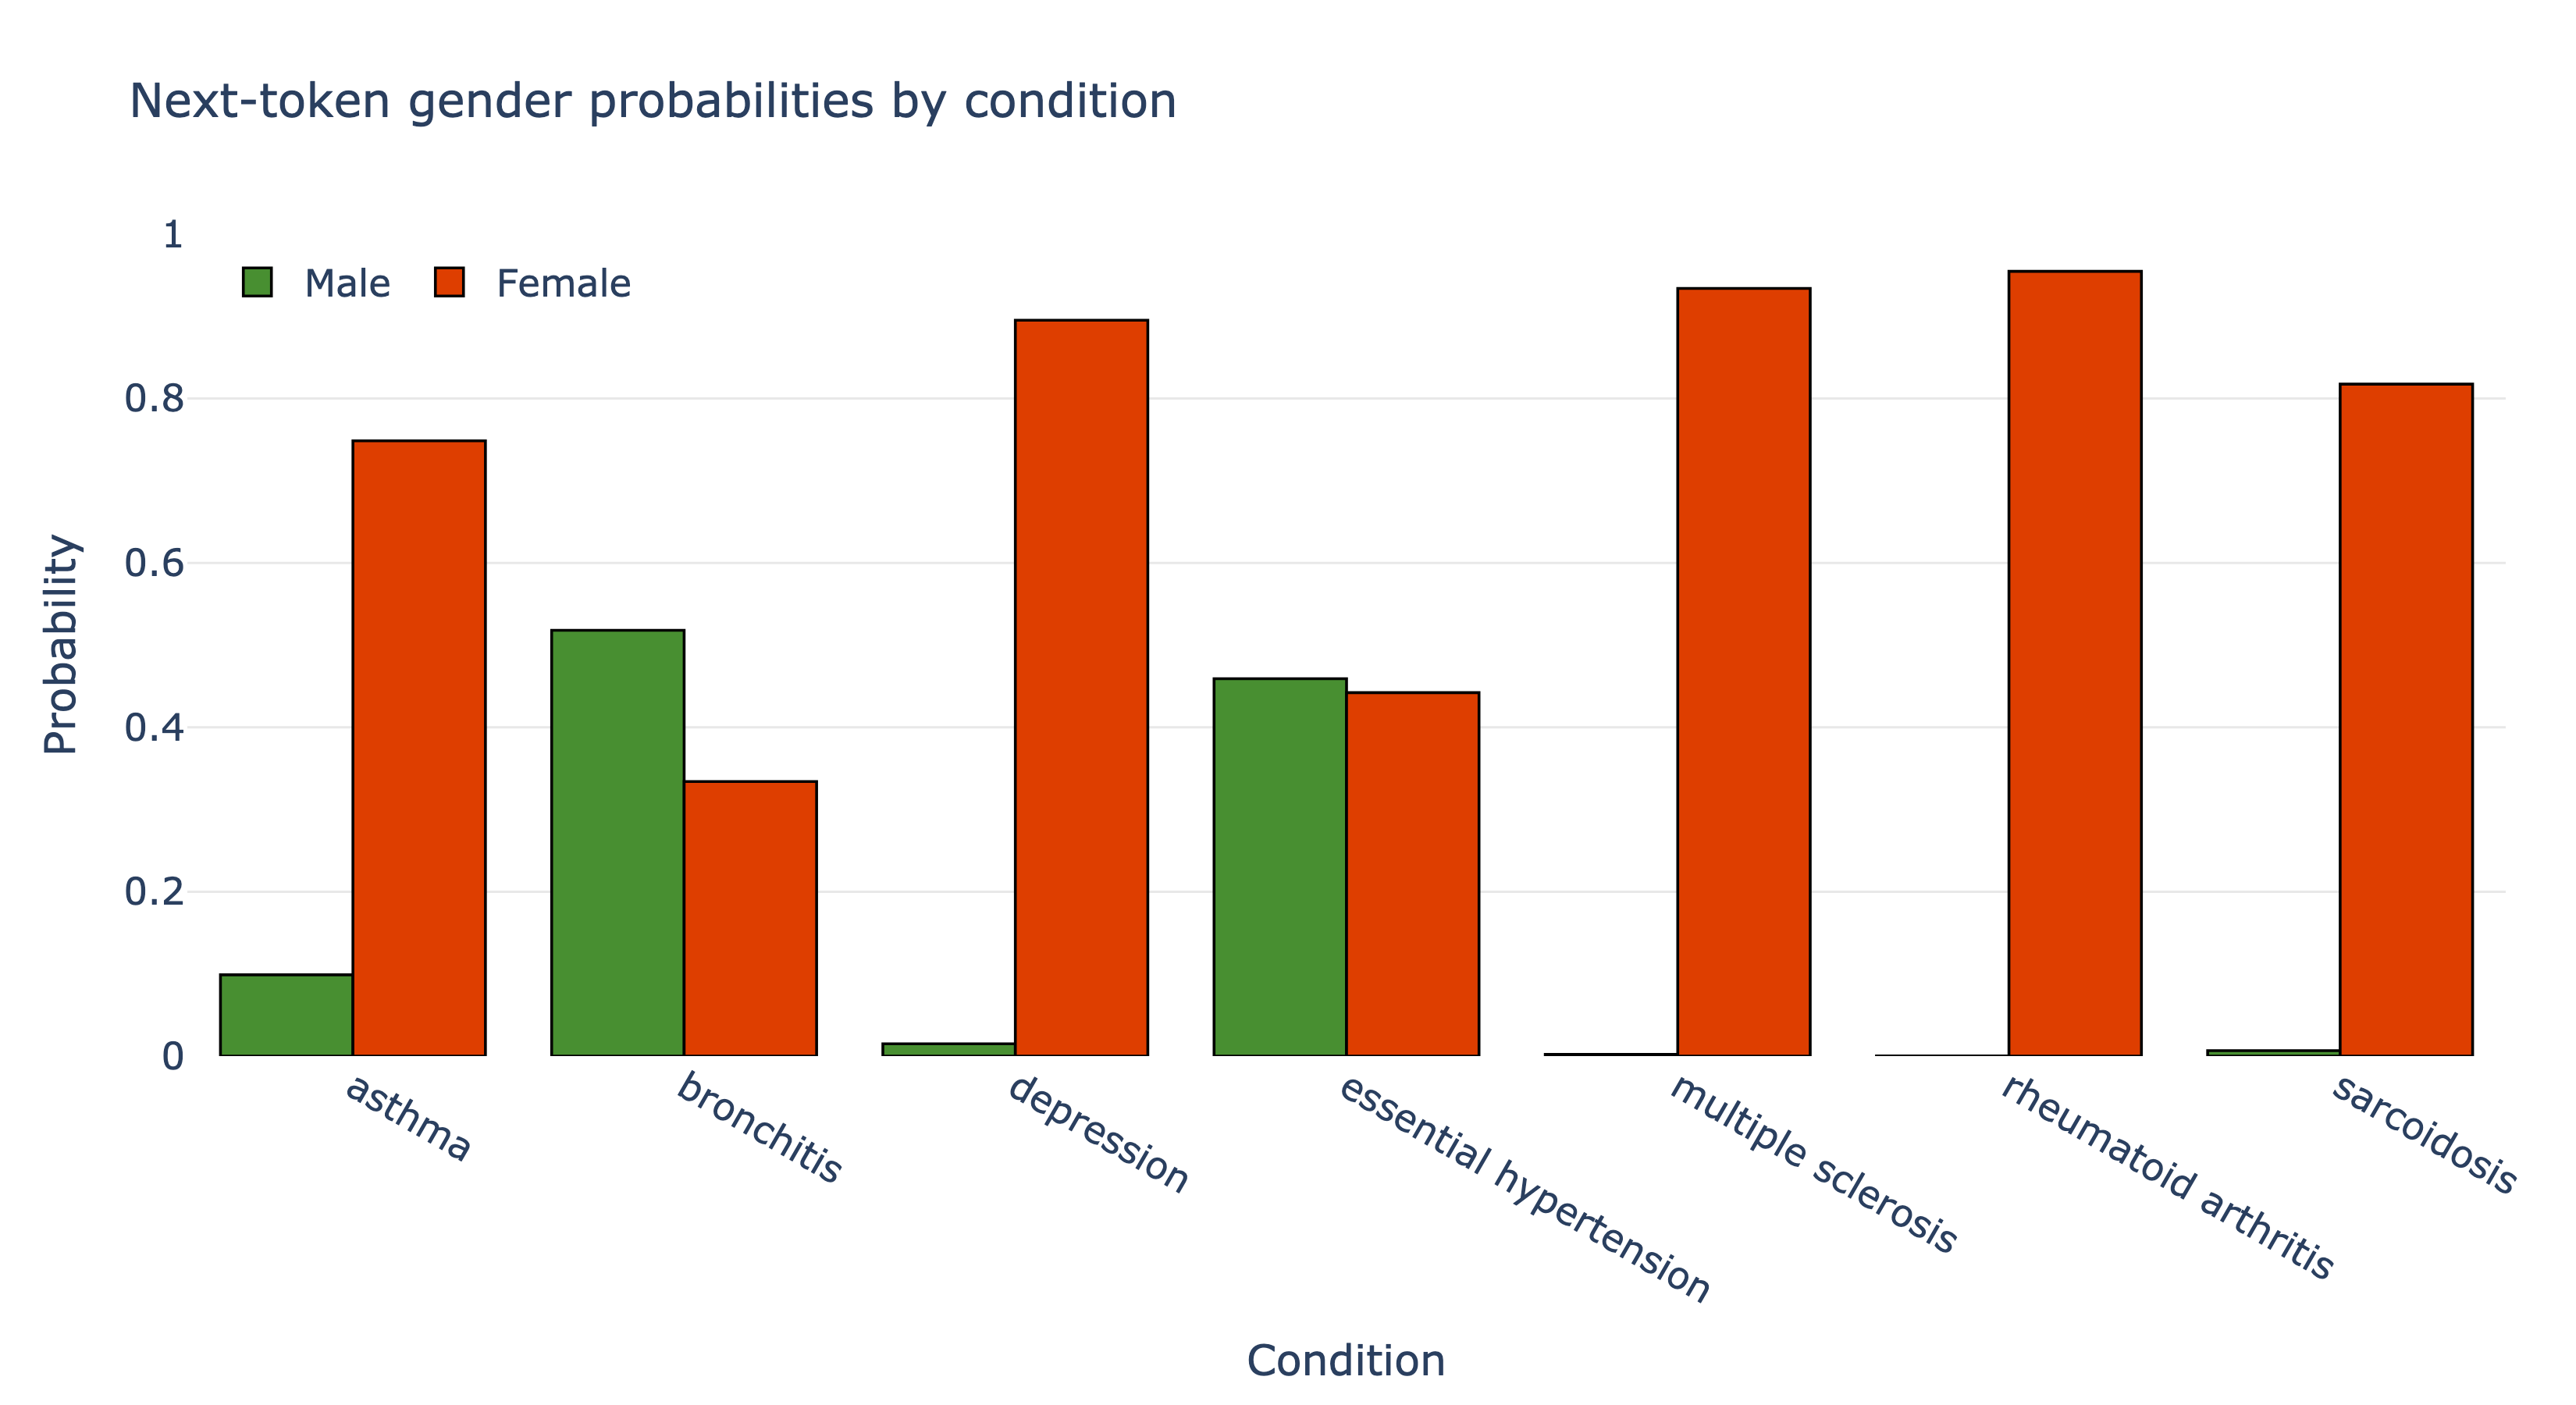
\includegraphics[width=1\linewidth]{fig1_gender_probs_by_condition.png}
    \caption{Proportion of male/female patients by condition and Qwen2.5-7B model for simple prompts.}
    \label{fig:prop}
\end{figure}

\begin{figure}[h]
    \centering
    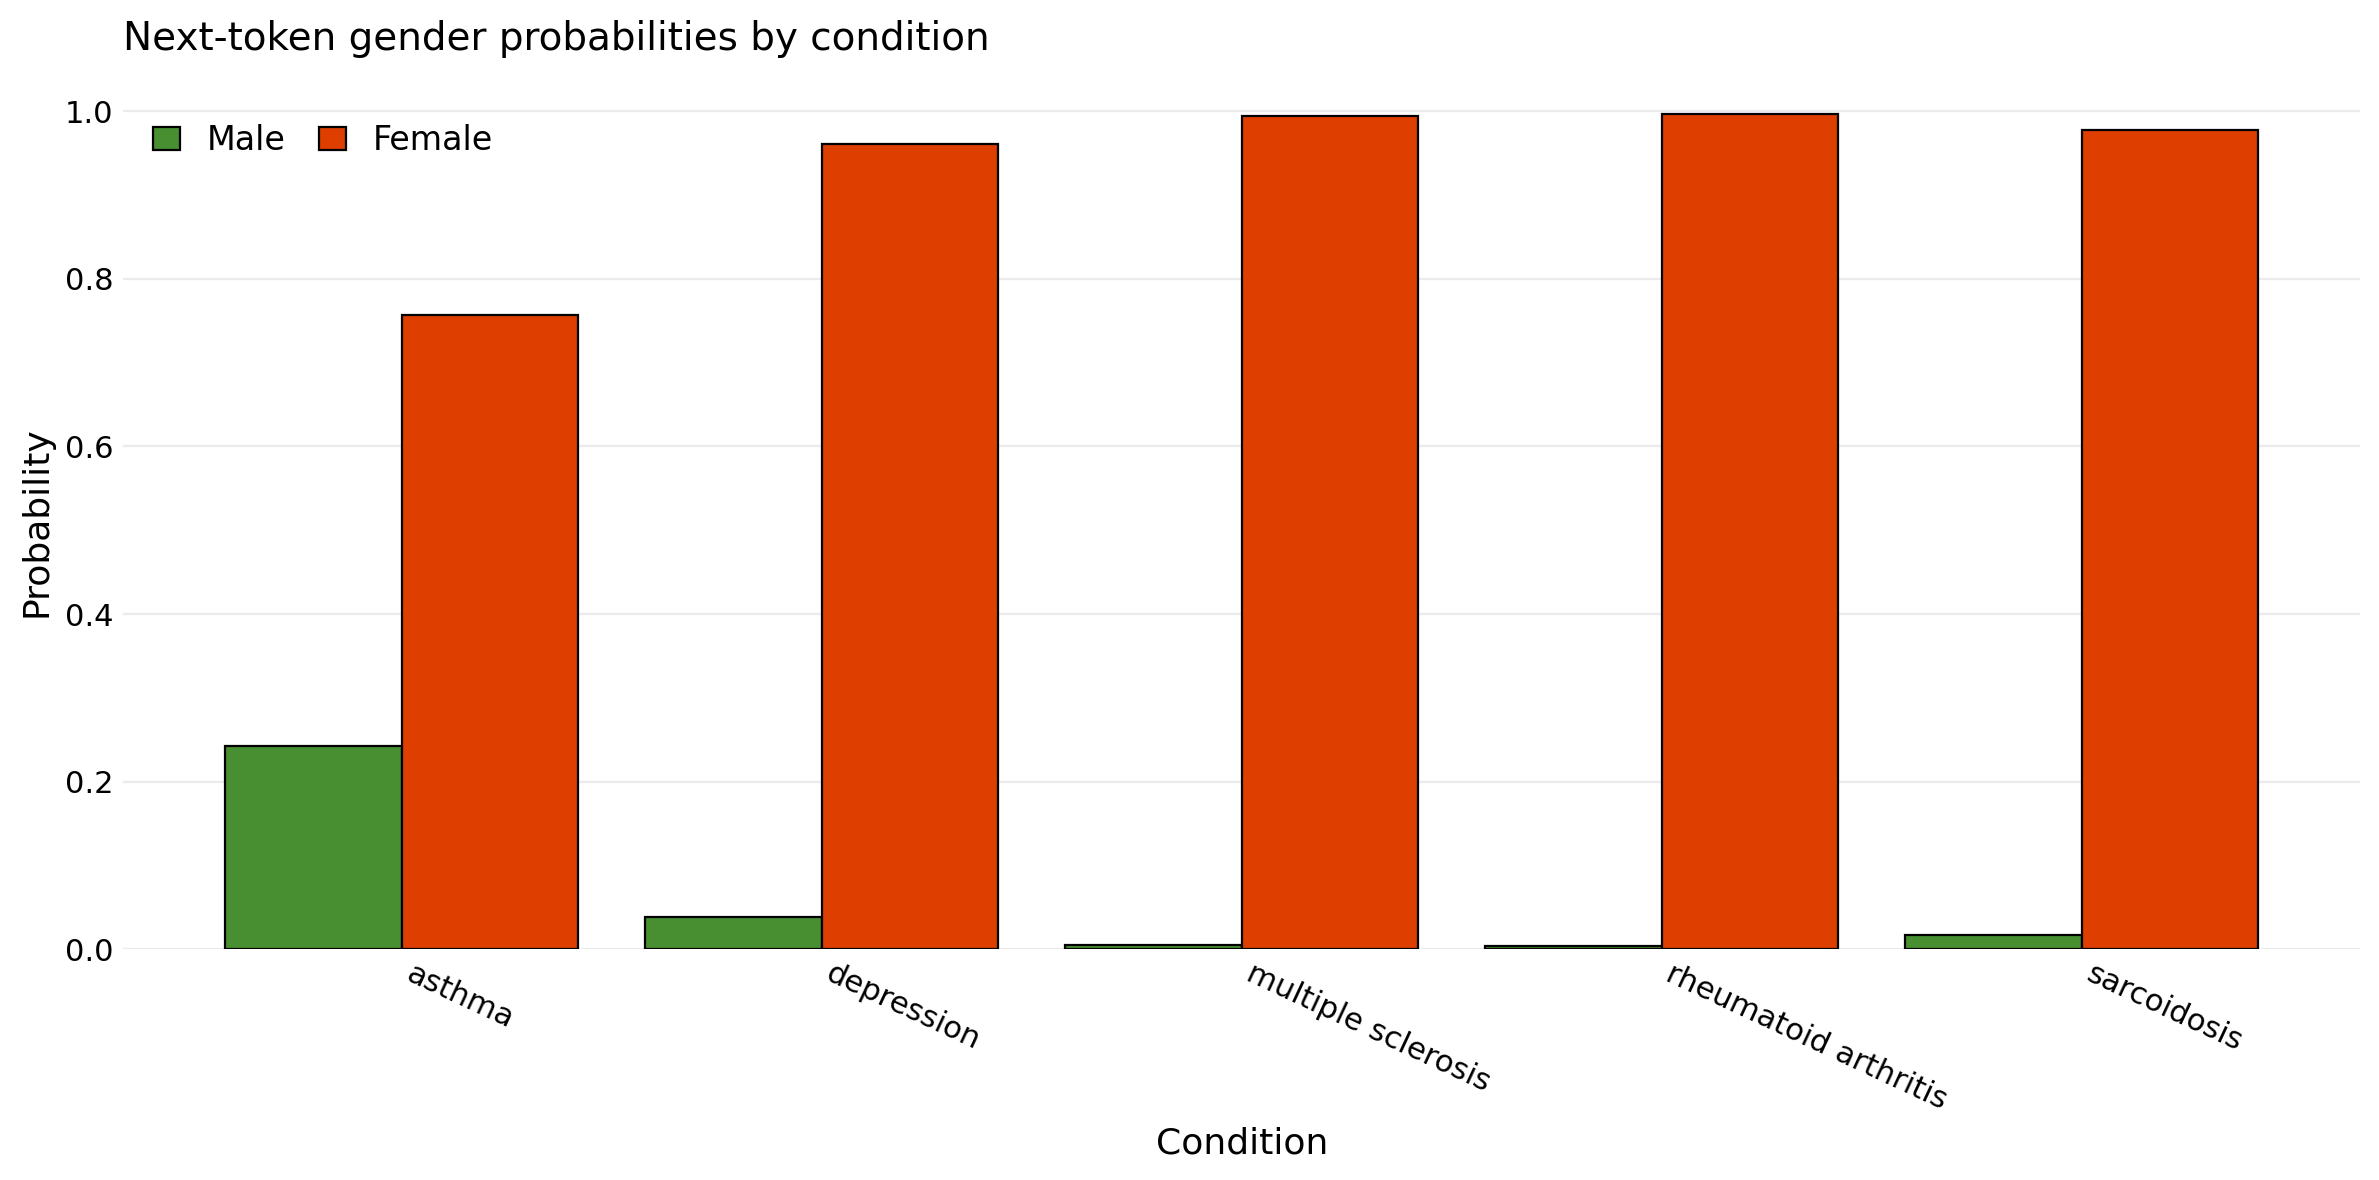
\includegraphics[width=1\linewidth]{fig1_gender_probs_by_condition_palette.png}
    \caption{Proportion of male/female patients by condition and Qwen2.5-7B model for CoT prompts.}
    \label{fig:cot_prop}
\end{figure}

\subsection{Activation Patching Setup}
For each target vignette prompt, we collect a source gender activation from a clean demographic prompt (e.g., ``The patient is Male'') and patch this activation into the target prompt at selected layer/token locations. We then measure the causal effect on male-token probability and downstream generated gender. Through our experiments we have ran full layer-token sweeps to map rewrite-score and logit-delta effects, then identify top localization layers. In our zero-indexed notation, Qwen's strongest non-artifact effects are centered at layer 18 (with nearby peaks), while OLMo shows a weaker but similarly positioned middle-layer peak. In addition, our results confirm that the rewrite score is focused on the respective layer and the last condition subtoken, supporting claims by (Ahsan et al. (2025); Marks and
Tegmark, 2023; Todd et al., 2023). 

\subsection{Simple-Prompt Results (Qwen + OLMo)}
In our experiments on Qwen, the strongest non-artifact effects are concentrated in middle layers. We consistently observe layer 18 as the most prominent, and Qwen shows clear internal localization of gender-sensitive effects in specific top layers. A recurring early-layer spike is treated as noise and excluded from interpretation. Experiments with OLMo display a similar general structure (including a middle-layer peak near layer 18), but with substantially smaller rewrite-score magnitudes. 

%need a figure here for aggregate rewrite score

\begin{figure}[h]
    \centering
    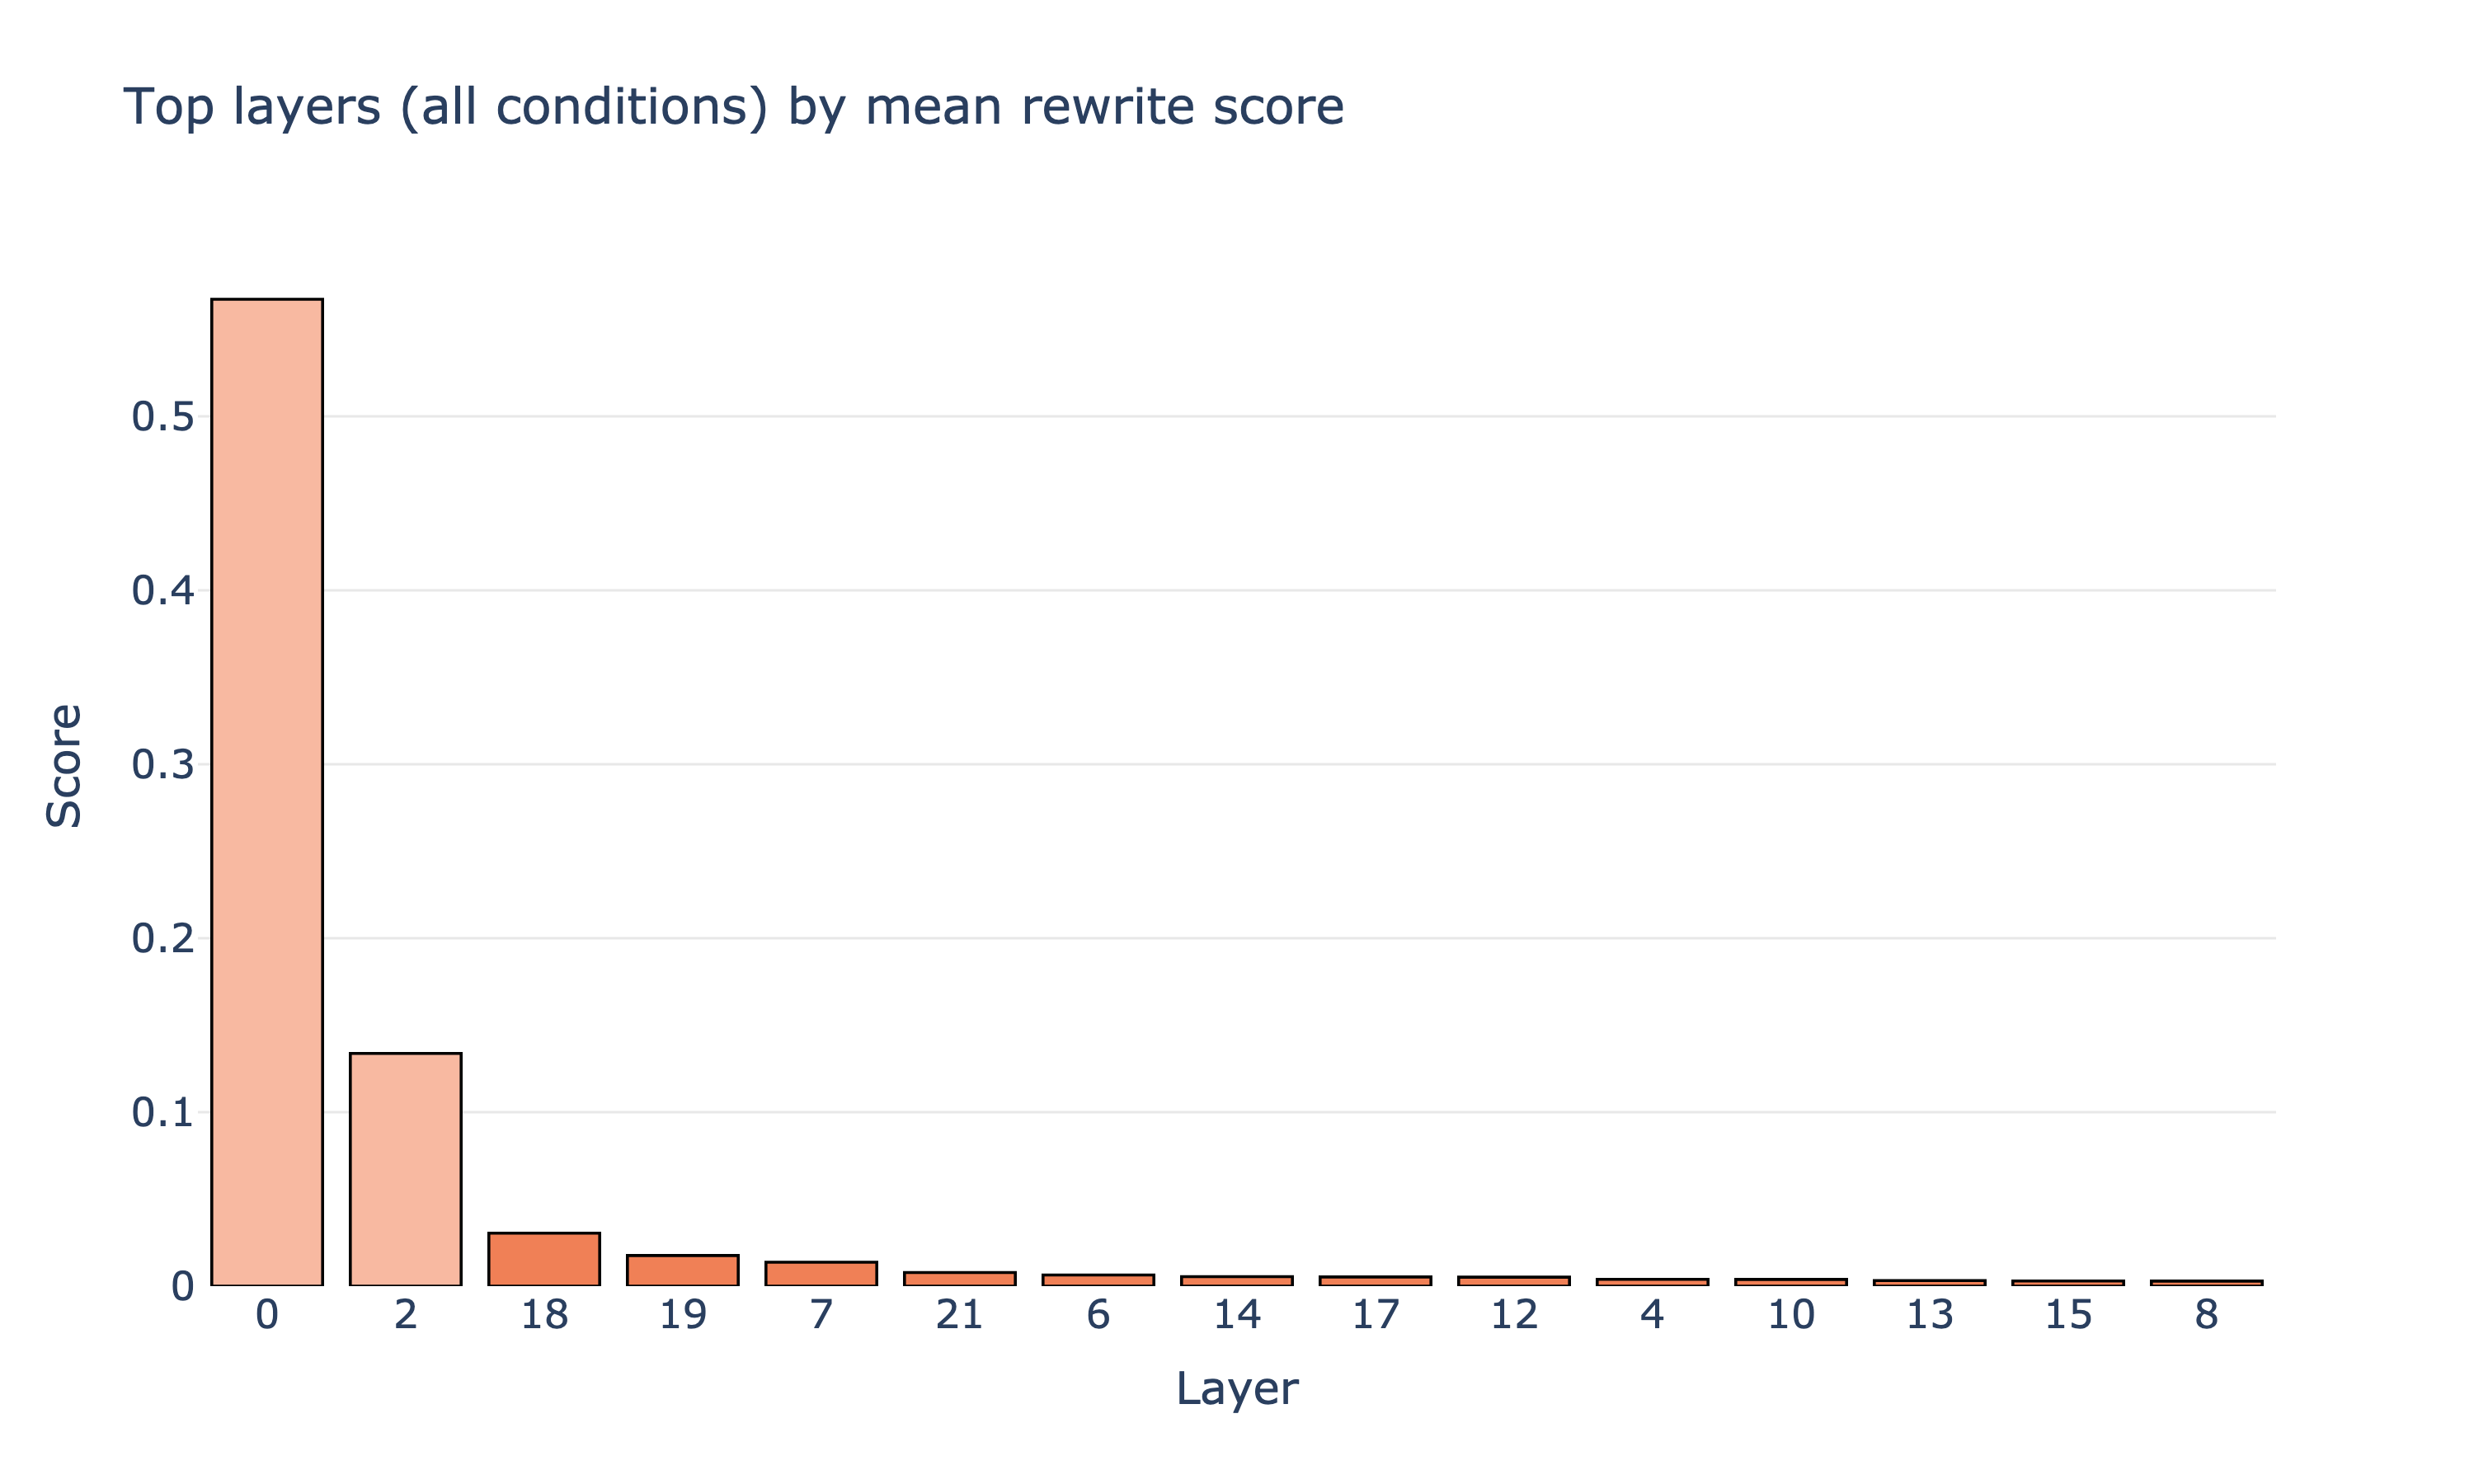
\includegraphics[width=1\linewidth]{fig2c_toplayers_all_conditions.png}
    \caption{Top Layers for Qwen Simple Prompting.}
    \label{fig:simpleaggregate}
\end{figure}

Analyzing results with a more granular (layer, token) pair, the rewrite score metric is much higher than the overall layer aggregate (Figure~\ref{fig:rewrite}), showing the localization of gender bias is highly localized to token association within each layer. This granular view still supports the magnitude difference of rewrite score between Qwen and OLMo model. This granular view also reveals the variation of rewrite scores based on condition. Asthma is highly malleable to patching while conditions like multiple sclerosis, rheumatoid arthritis, and sarcoidosis show very low rewrite scores.

\begin{figure}[h]
    \centering
    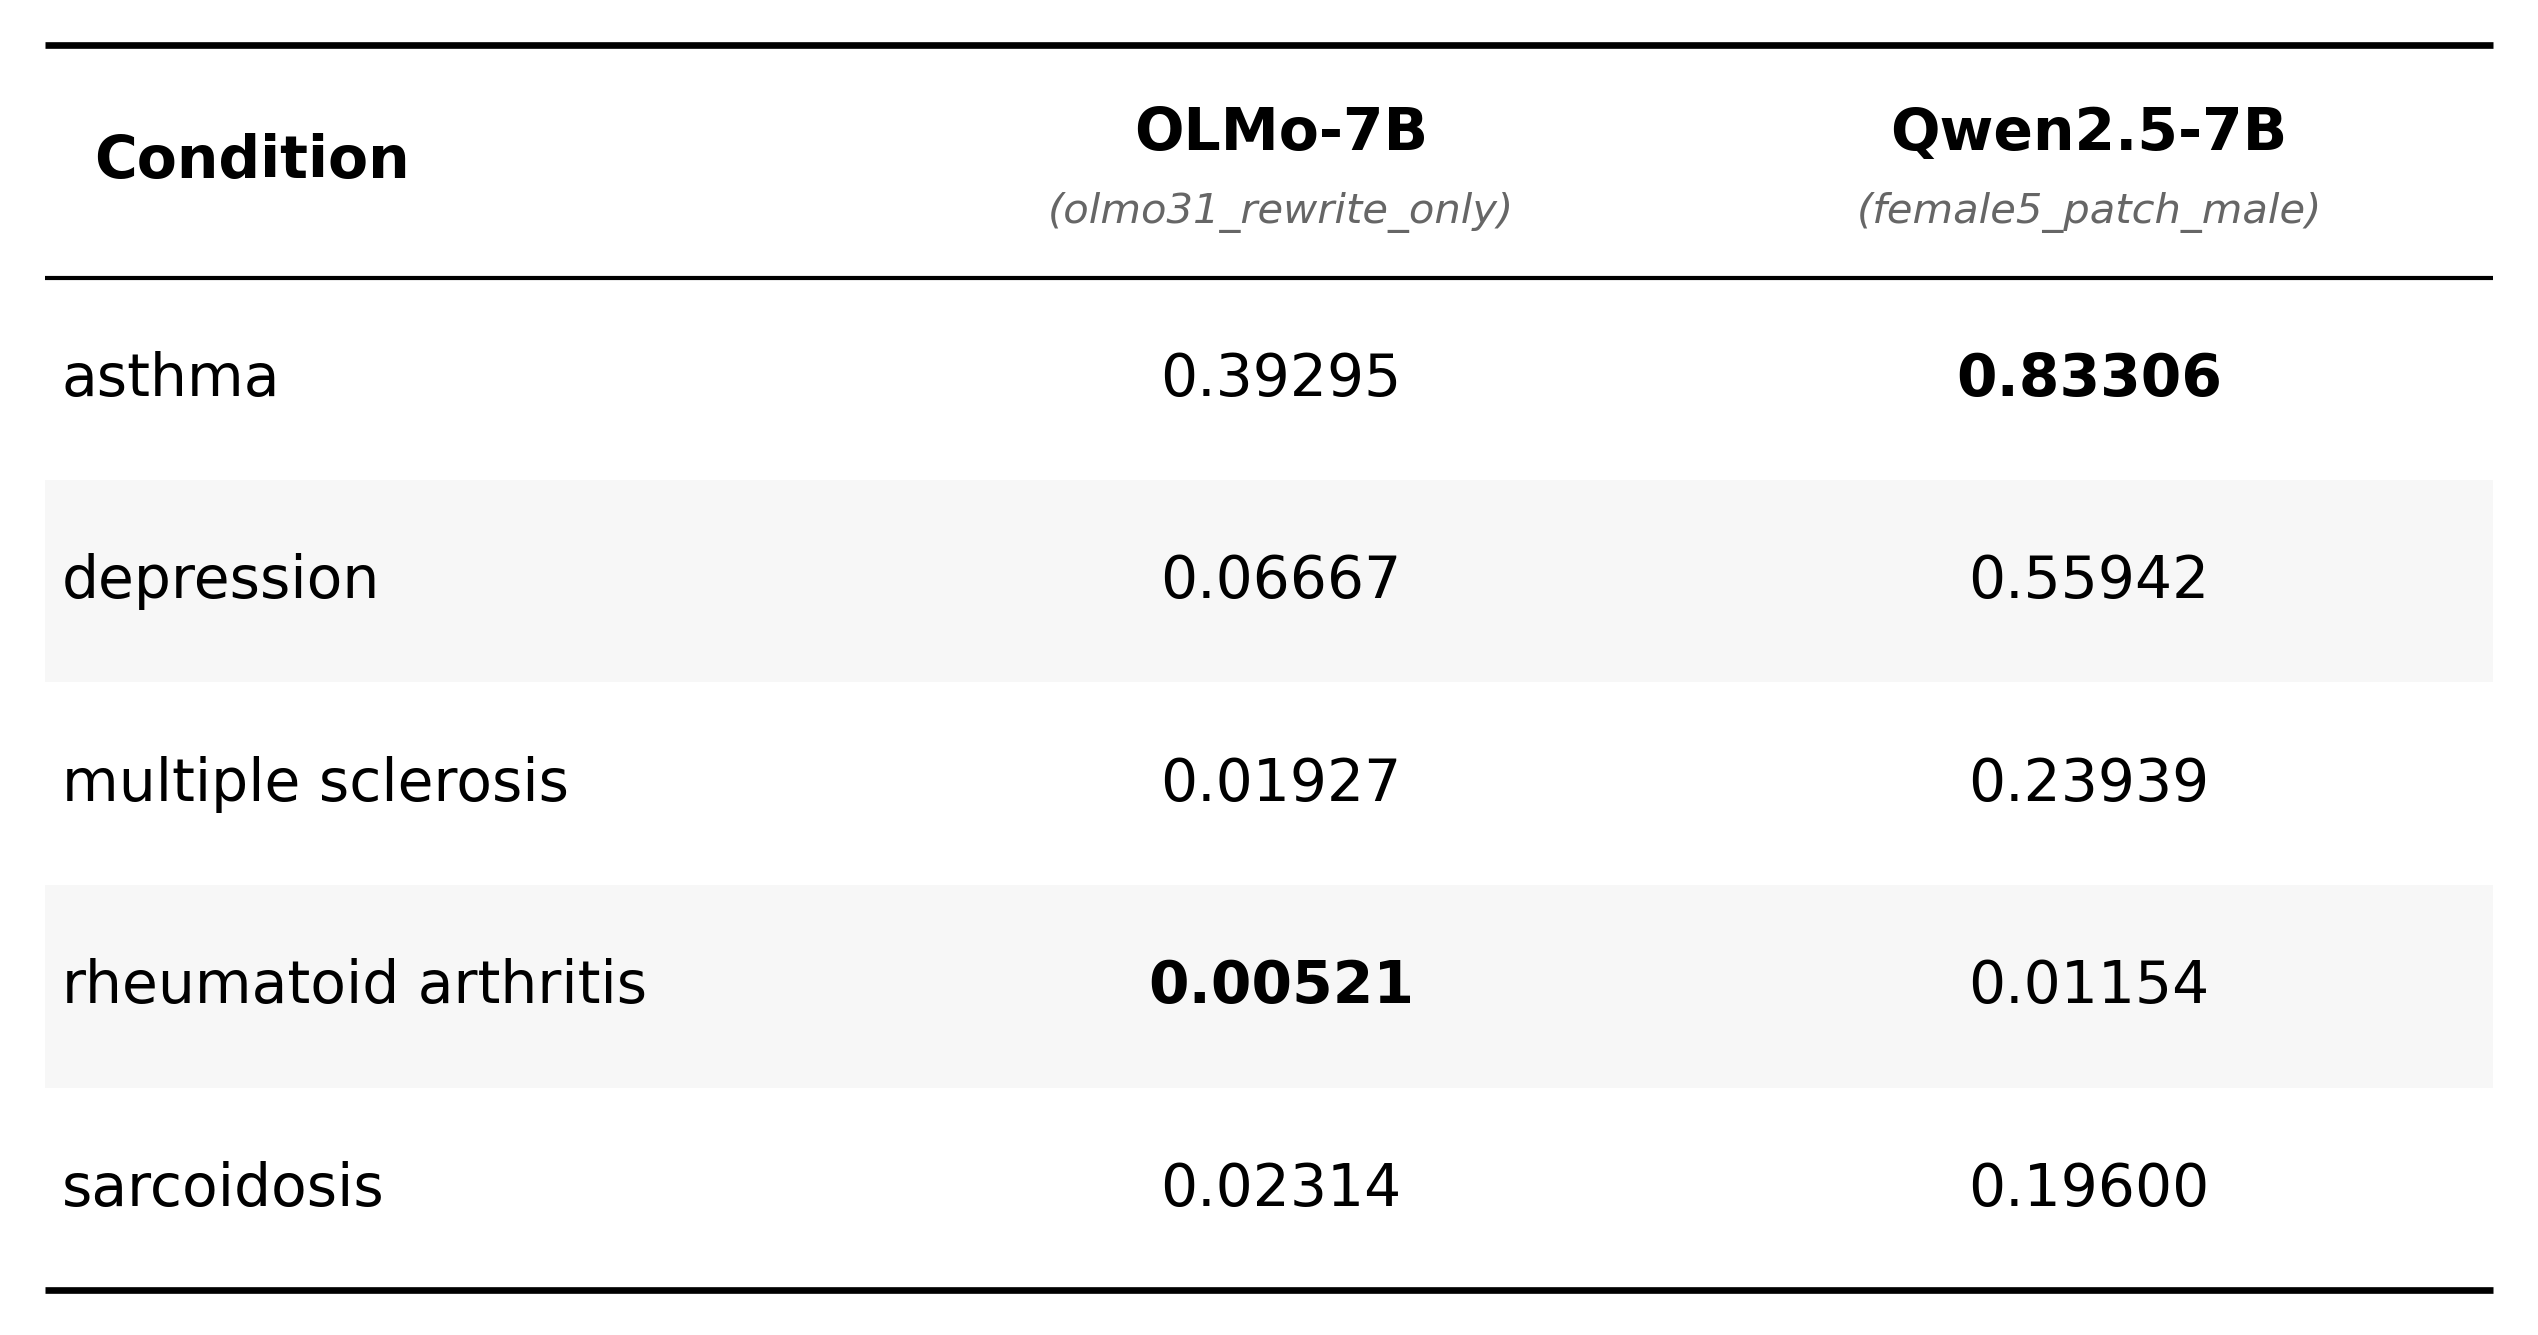
\includegraphics[width=1\linewidth]{fig2_token_association_table.png}
    \caption{Rewrite score of simple activation patching in layer 18 and condition-token pair.}
    \label{fig:rewrite}
\end{figure}


This disparity in rewrite score across conditions can be further seen by analyzing the specific prompt, condition heatmaps. Figure~\ref{fig:heatmap} Results for asthma across all 31 prompts show similar results, strong localized activation at layer 18 that is associated with the condition token. On the other hand, results from rheumatoid arthritis show little to no rewrite score changes in any of the middle layers. Our findings show the internal encodings of gender bias are not uniform across all female biased diseases. The data displays the disparity in how easily difference biases can be patched. 


\begin{figure}[h]
    \centering
    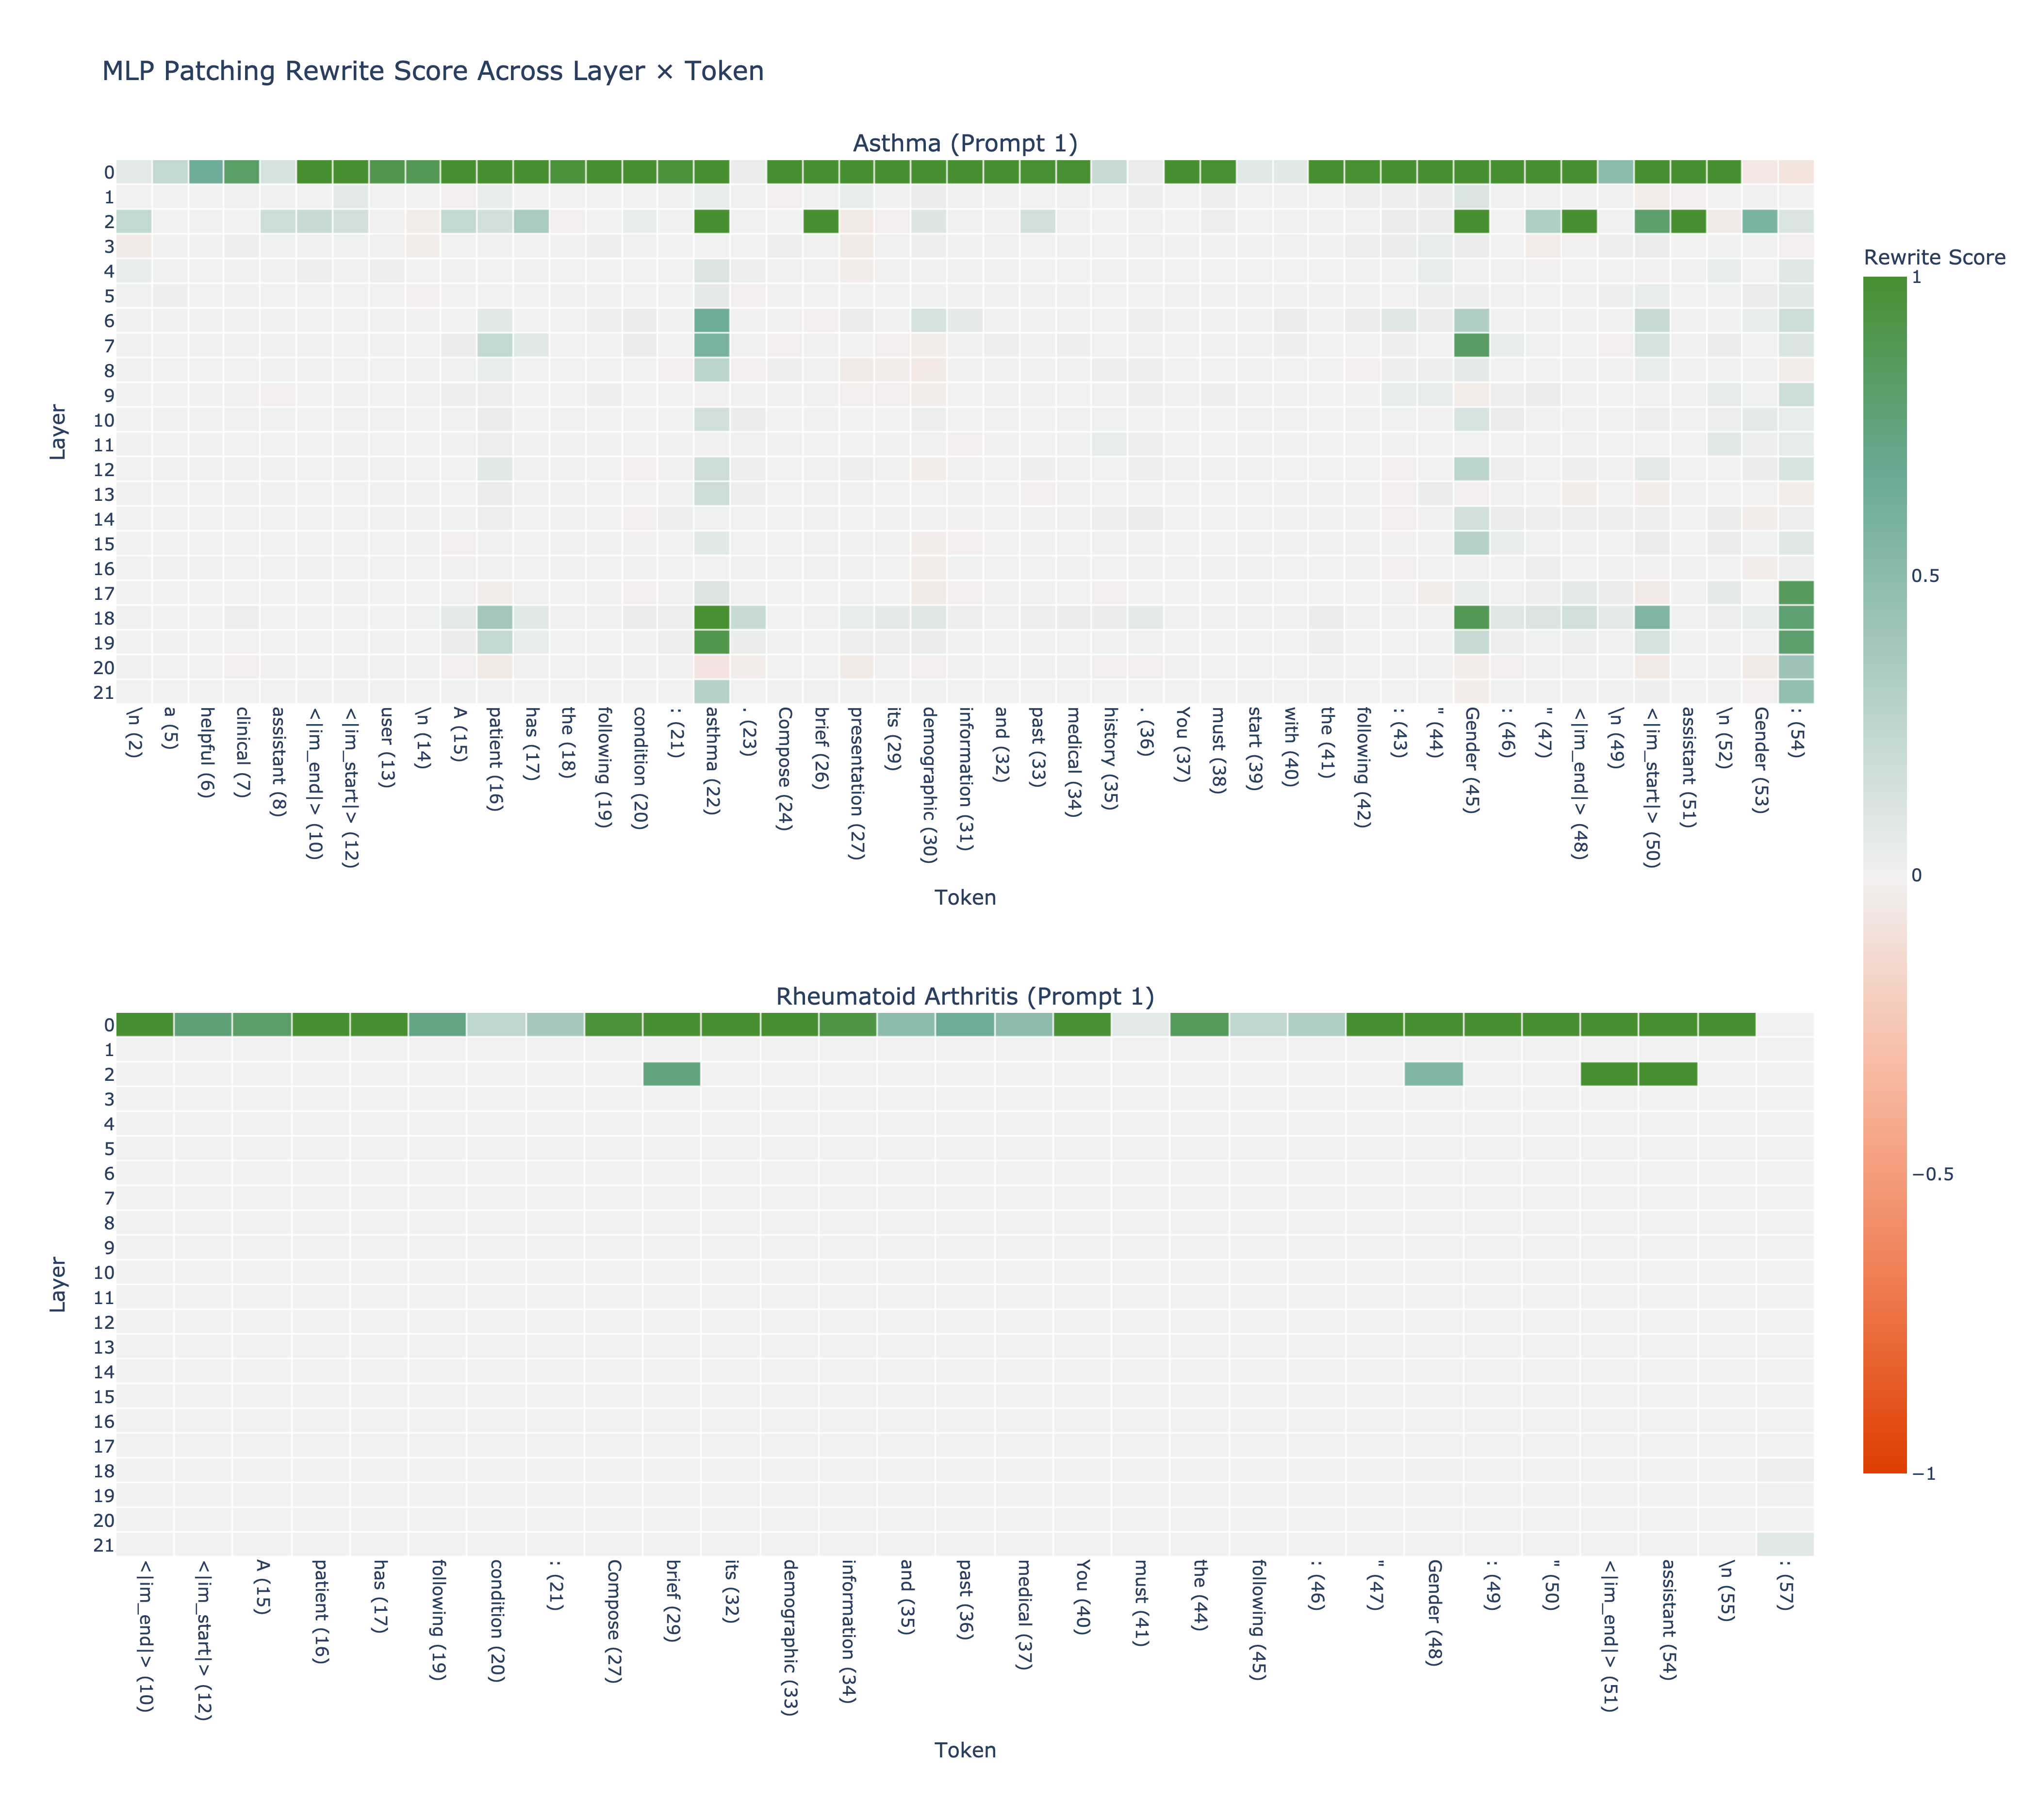
\includegraphics[width=1\linewidth]{fig5_mlp_heatmaps_combined_asthma_ra.png}
    \caption{Qwen simple-prompt MLP patching heatmap (rewrite score) across layer $\times$ token for representative asthma and rheumatoid-arthritis prompts.}
    \label{fig:heatmap}
\end{figure}

We further evaluated activation patching by measuring its ability to alter gendered generations across multiple medical vignette prompts and cohorts. Extending prior activation patching studies, we find that intervention effectiveness is highly sensitive to both prompt structure and underlying cohort-specific bias.

To better capture these distributional effects, we additionally reran portions of the simple patching experiments using a log-delta metric in place of the rewrite score used in prior work. We find that log-delta more reliably captures small but systematic shifts in gendered output probabilities, particularly in regimes where rewrite score is less sensitive to subtle distributional changes. Overall, these results indicate that conclusions regarding the robustness of activation patching depend critically on prompt selection, cohort composition, intervention magnitude, and evaluation metric choice. These behavioral shifts are consistent with our earlier localization results, suggesting that interventions targeting middle-layer representations causally influence downstream gendered generation behavior.


\subsection{Model Comparison}
Building on the per-condition results in Section 2.3, we compare how the two models localize patient gender under simple prompting, using two metrics. The rewrite score is the probability-space metric defined in the methods. The logprob delta is an unbounded log-probability metric used alongside it. We utilized logprob delta metric because of less saturation in extremes and added stability for tiny probabilities, which was common in our findings.

%our results is seriously messed up in this section will have to come back later

On the rewrite score, both models place their strongest non-artifact effect at layer 18, Qwen at 0.398 and OLMo at 0.130. The logprob delta sharpens this: rheumatoid arthritis looks near-unresponsive on the rewrite score (0.012) but has a layer-18 logprob delta in the same range as the other conditions, so its near-zero rewrite score is a saturation artifact rather than evidence of an absent gender circuit. 

We also ran the simple-prompt sweep at the residual-stream site for Qwen: rather than a sharp layer-18 peak, residual patching produces a broad mid-layer plateau spanning roughly layers 5 through 21, then collapses sharply to near zero at layer 22. The layer-18 MLP feature is best read as a concentrated readout within a broader distributed residual representation.

\subsection{Residual Stream Patching}

To complement the MLP localization, we ran the simple-prompt sweep at the residual-stream utilizing Qwen, across the same five cohorts and 31 prompts. 

Rather than a sharp layer-18 peak, residual patching produces a broad mid-layer plateau. After excluding the early chat-template layers (layers 0 to 4), which carry no localization claim, the plateau spans roughly layers 5 through 21 with mean rewrite scores around 0.8 to 0.94, then collapses sharply to near zero at layer 22. Although results of the two sites seem contradictory, MLP patching isolates a specific sublayer's nonlinear computation and finds a concentrated layer-18 feature, while residual patching replaces the entire accumulated hidden state and registers gender information across many layers at once. As a result, the layer-18 MLP feature is best read as a concentrated readout within a broader distributed residual representation.

\begin{figure}[h]
    \centering
    
\includegraphics[width=1\linewidth]{fig11_residual_plateau_qwen.png}
    \caption{Per-layer Rewrite score for Simple-Prompt Residual Patching in Qwen. 
}
    \label{fig:resdstream}
\end{figure}


\subsection{Mechanistic Analysis: CoT Setup}
The key extension of this paper is moving from simple prompting to CoT prompting in the same mechanistic framework. Prior work established localization under simple prompts, and we test whether CoT changes internal gender processing. Specifically, we compare (1) localization location, whether the same layers carry the gender signal or it shifts and (2) localization concentration, whether the signal remains localized or becomes distributed.

We applied the same activation-patching framework from Section~2.2 to CoT-prompted generations, run on both Qwen2.5-7B-Instruct and OLMo-7B-Instruct. There is one way in which the CoT setup differs from simple prompting: we patch across the full frozen input, meaning the original prompt plus the appended reasoning trace, rather than patching directly at the final gender token. This lets us target condition-token positions across every layer, so any gender signal that has migrated into the reasoning trace is captured, and allows us to evaluate whether CoT produces genuine internal debiasing or only changes the surface form of reasoning. Example traces can be seen in (Appendix Table 1)

\subsection{Mechanistic Analysis: CoT Results}
\paragraph{MLP intervention.} Under CoT, MLP layer-18 rewrite scores at the \emph{first} condition token remain strong and comparable to simple prompting (Qwen: $\sim$0.44 vs $\sim$0.40). Scores at later condition mentions in the same trace are much weaker ($\sim$0.05). Thus CoT does not erase the early condition-token layer-18 effect; the effect is concentrated early and weaker later. We therefore report first- vs last-condition-token scores as the primary CoT MLP statistic, rather than treating sparse heatmap cells as evidence that the circuit disappeared (Figure~\ref{fig:cotmlp}).


The grid averages do hide a sparse surviving signal, but it is weak and is organized differently in each model. For OLMo, the cells that exceed a rewrite score of 0.1 sit mostly at layer 18 and are dominated by essential hypertension under Prompt C. For Qwen, the surviving cells are more numerous but spread across early and middle layers, with layer 2 contributing the most, and they are dominated by depression and asthma under Prompt C while other conditions show no signal.

Where simple-prompt MLP patching localized a gender effect at layer 18 consistently across conditions and across both models, CoT MLP patching leaves only a weak, prompt-specific, and model-specific remainder that does not average into a consistent circuit (Figure~\ref{fig:cotmlp_var}). These results stand in sharp contrast to simple prompting, where the layer-18 MLP peak was clear in both models (Qwen 0.398, OLMo 0.130).

\begin{figure}[htbp]
    \centering
    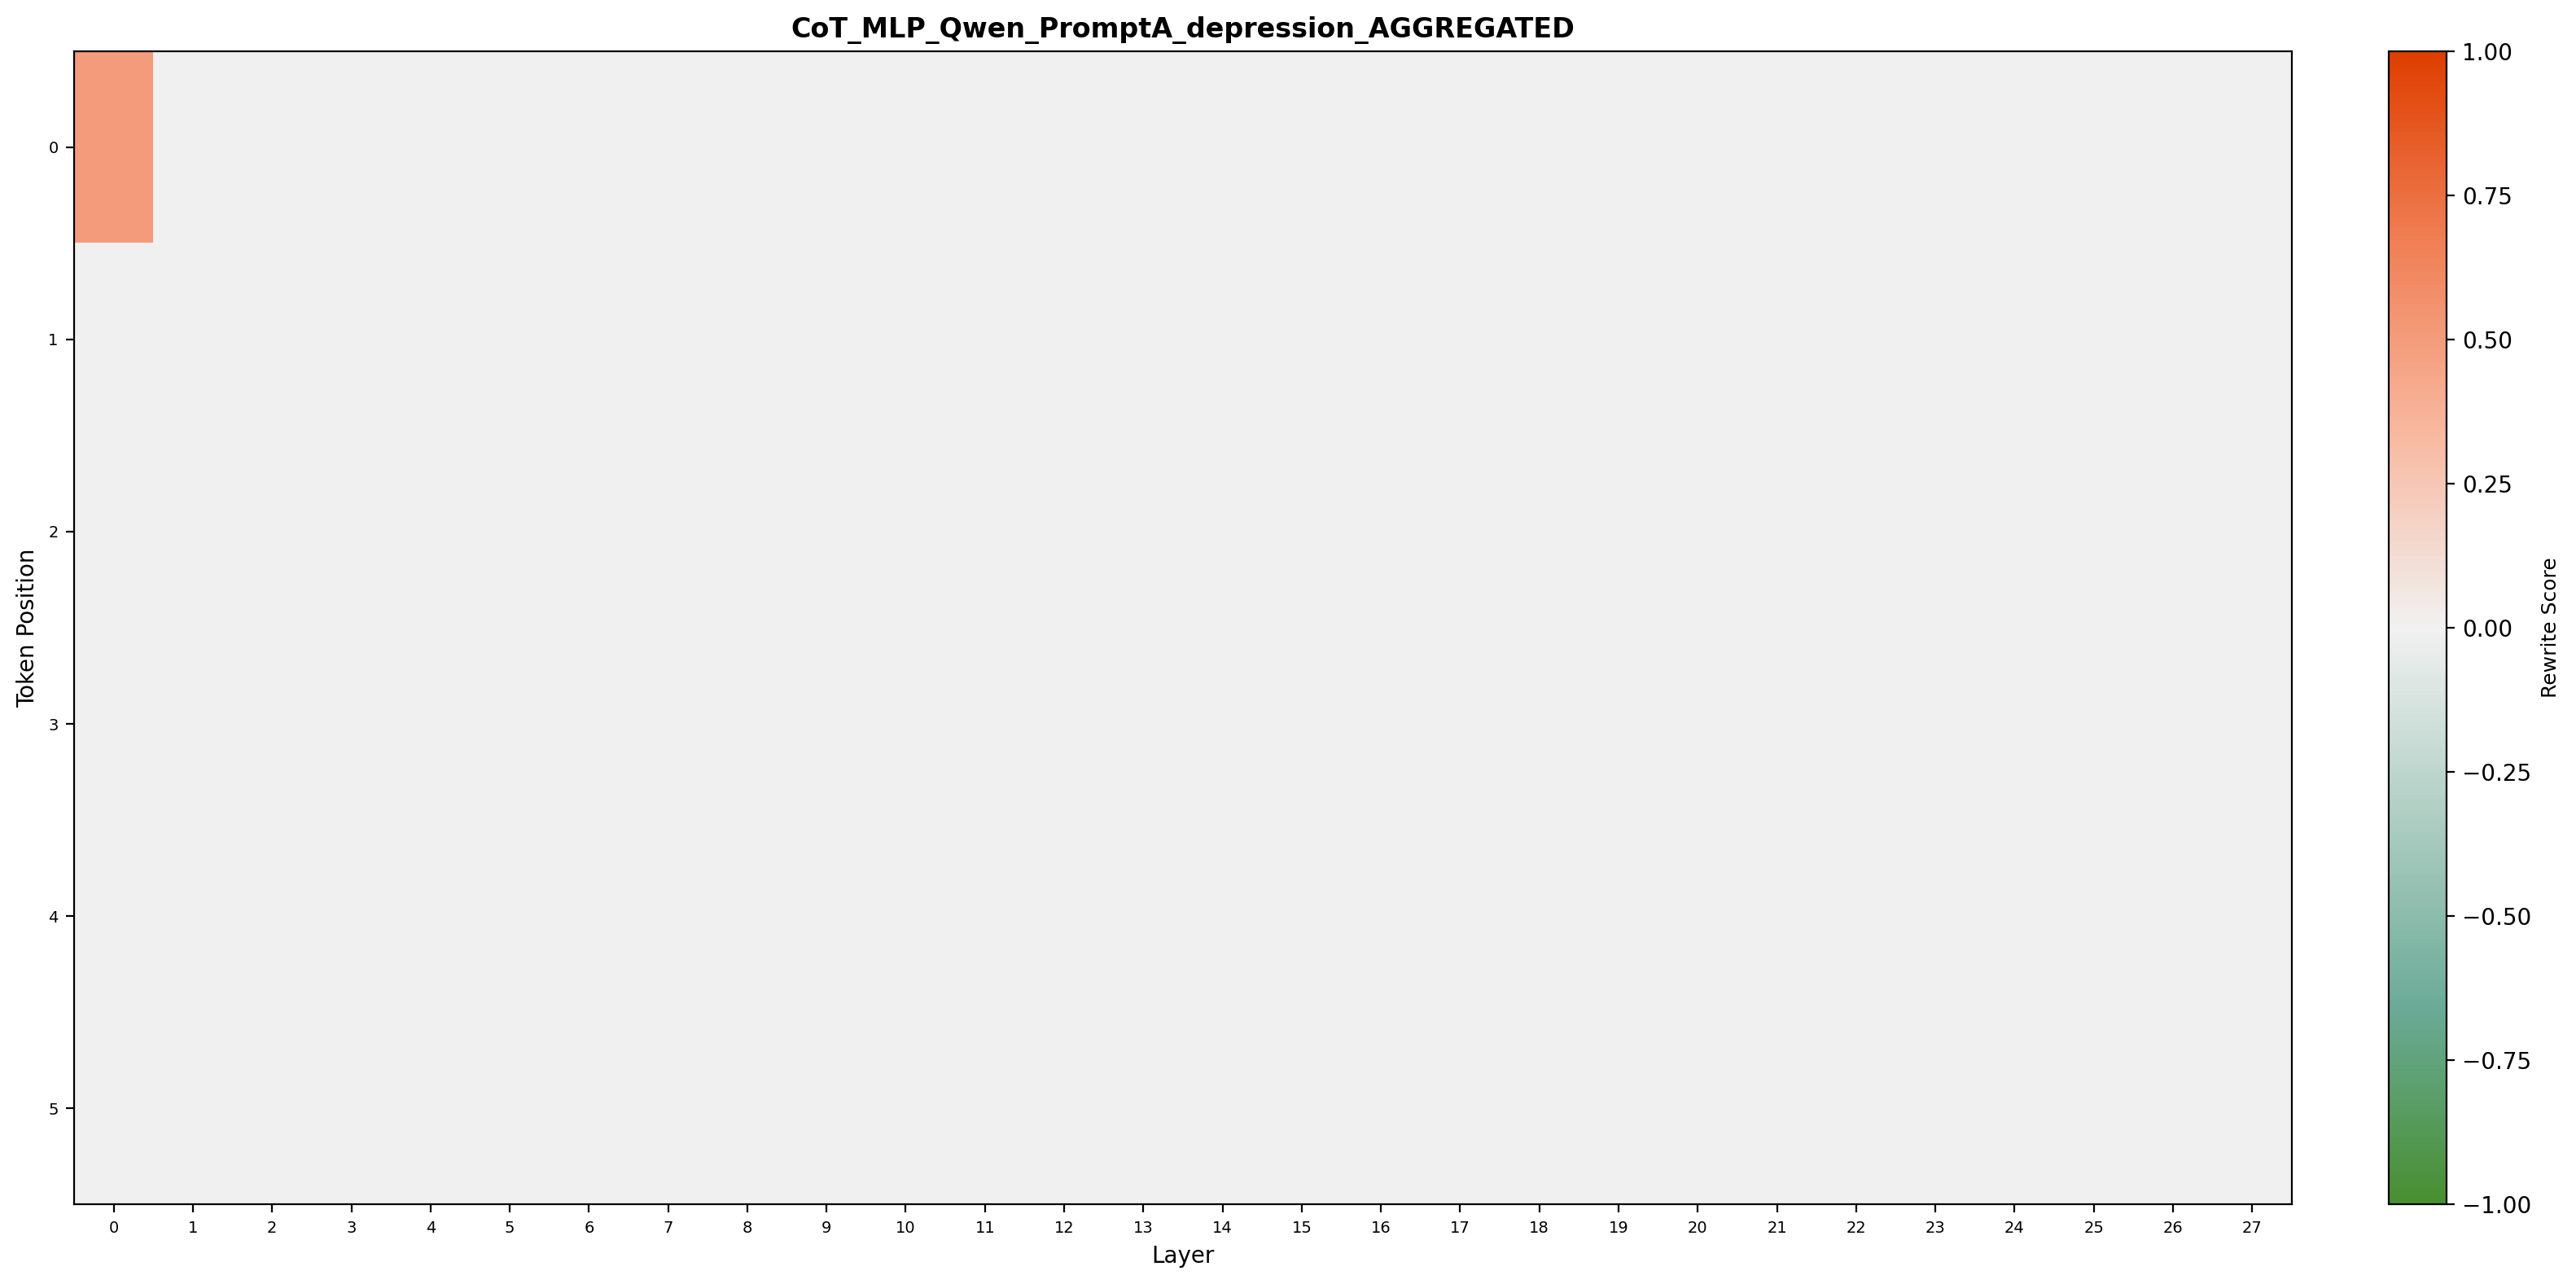
\includegraphics[width=1\linewidth]{CoT_MLP_Qwen_PromptA_depression_AGGREGATED.png}
    \caption{Representative CoT MLP Qwen Prompt A rewrite-score heatmaps. Other conditions removed for brevity but representative of other conditions.}
    \label{fig:cotmlp}
\end{figure}


\begin{figure}[h]
    \centering
    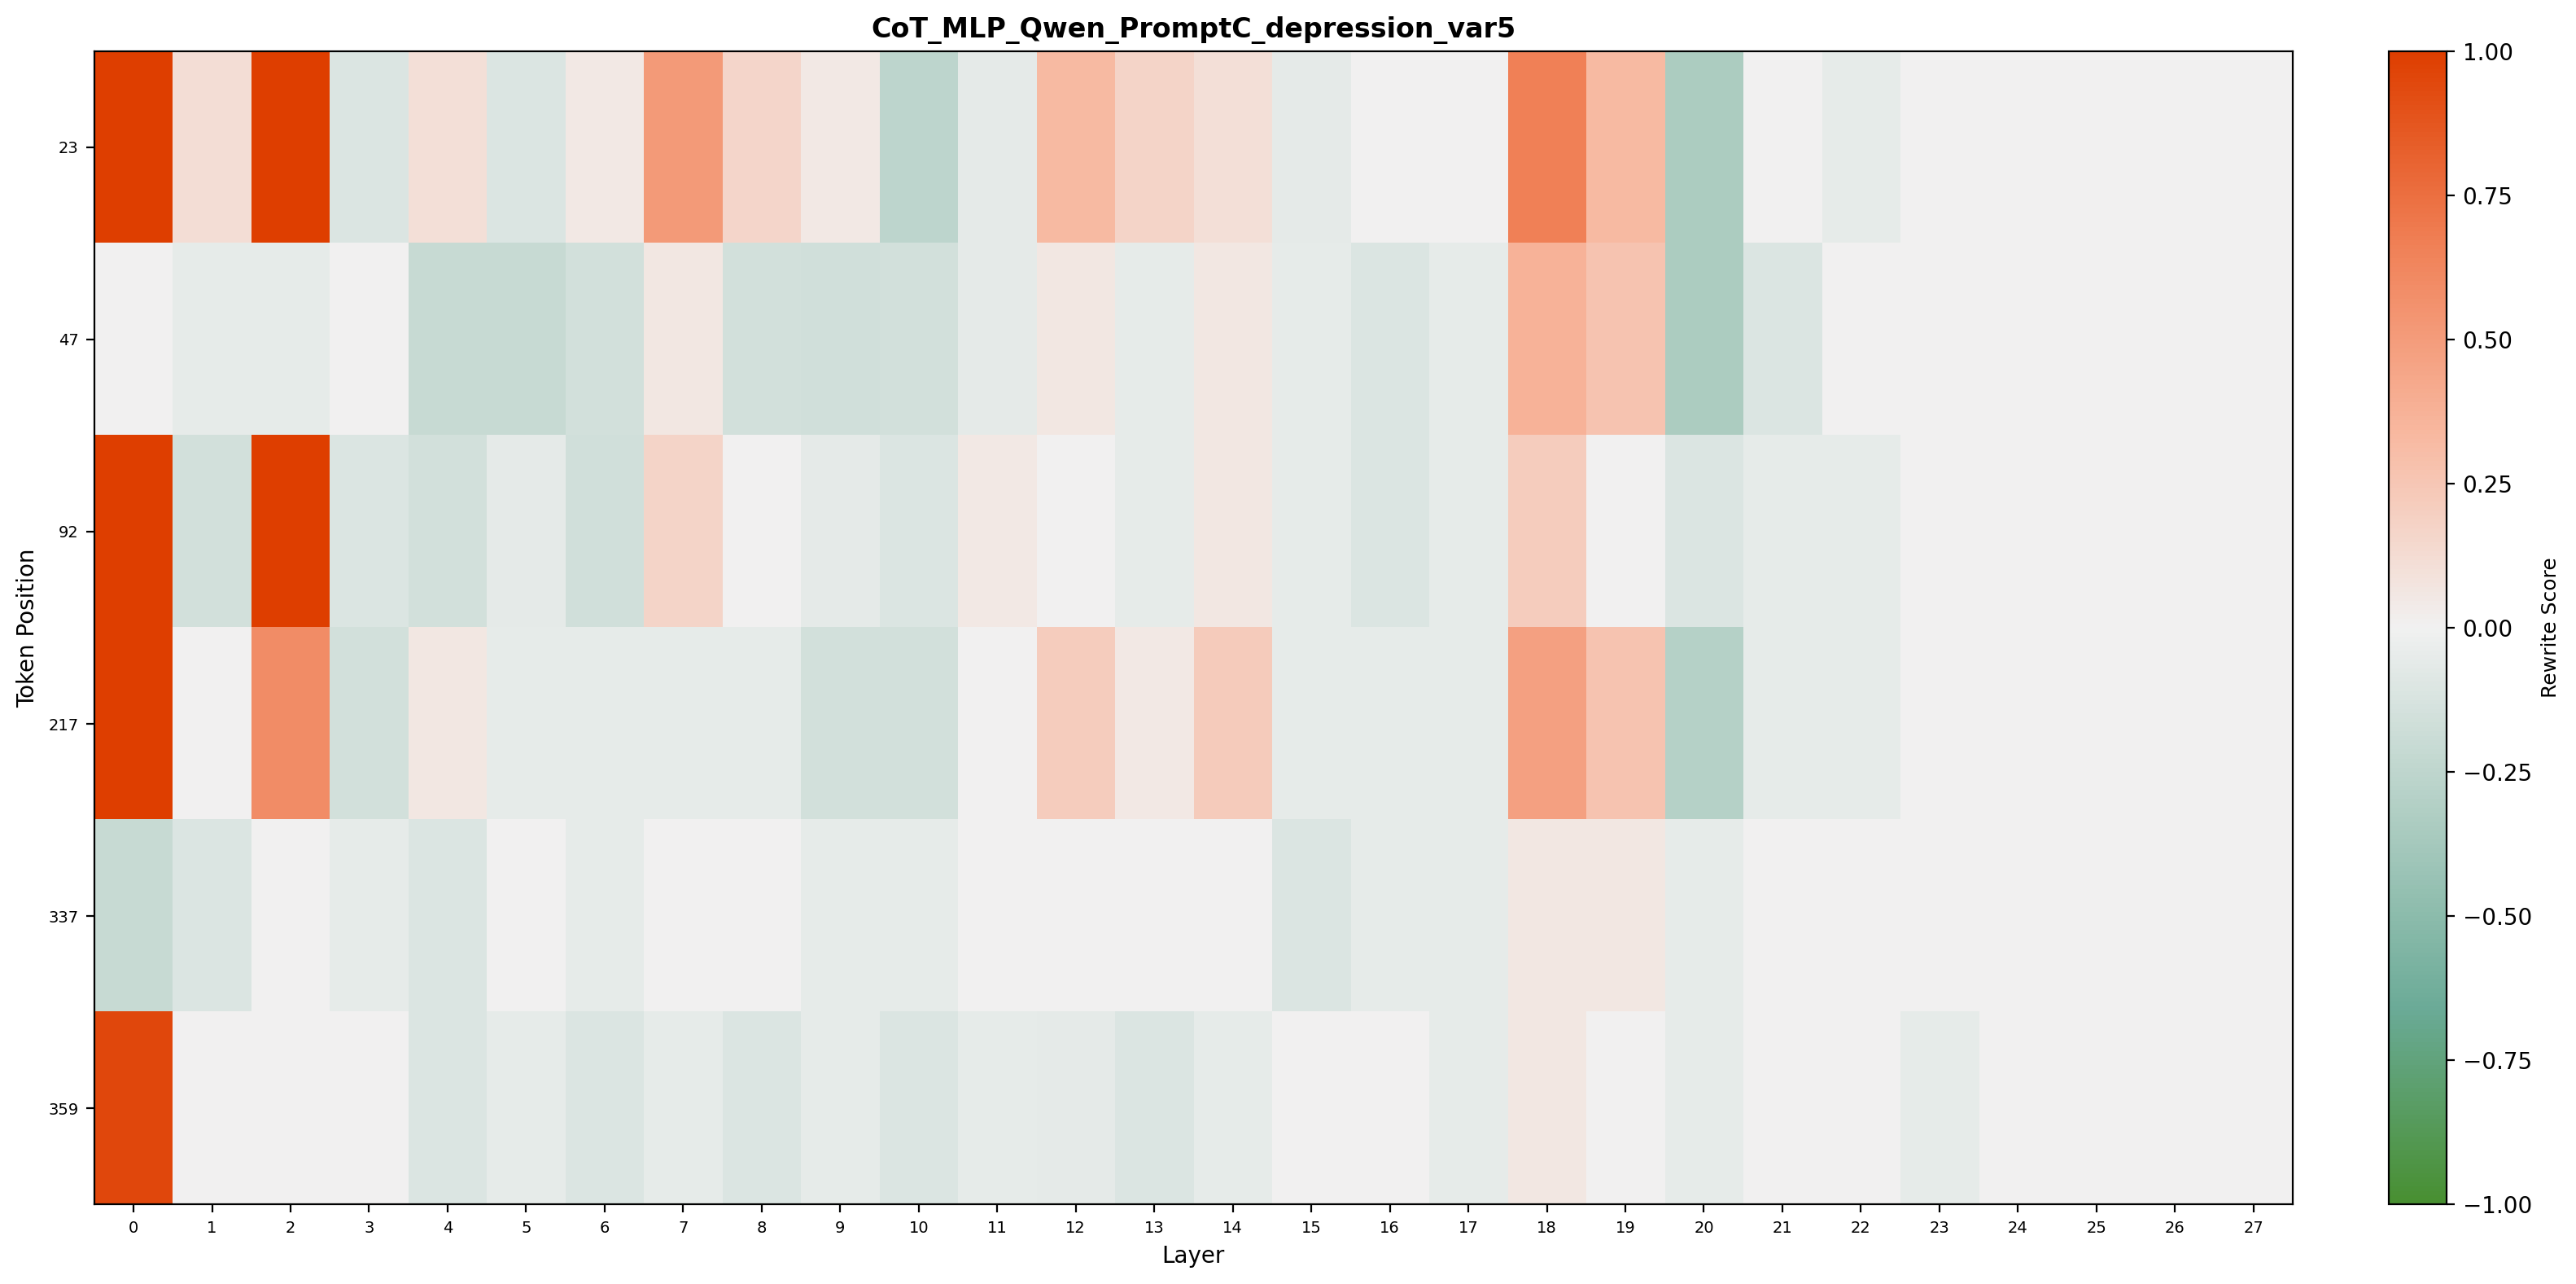
\includegraphics[width=1\linewidth]{CoT_MLP_Qwen_PromptC_depression_var5.png}
    \caption{Representative Prompt Specific Outlier from Prompt C.}
    \label{fig:cotmlp_var}
\end{figure}

\paragraph{Residual-stream intervention.} Residual-stream patching under CoT produces a different pattern: positive rewrite scores appear broadly across tokens and layers rather than at a single layer, spanning roughly layers 1 through 20 before approaching zero from about layer 22 onward (Figure~\ref{fig:cotresid}). Under CoT, gender-related information appears distributed across much of the accumulated residual representation rather than localized to a narrow region.

\begin{figure}[ht]
    \centering
    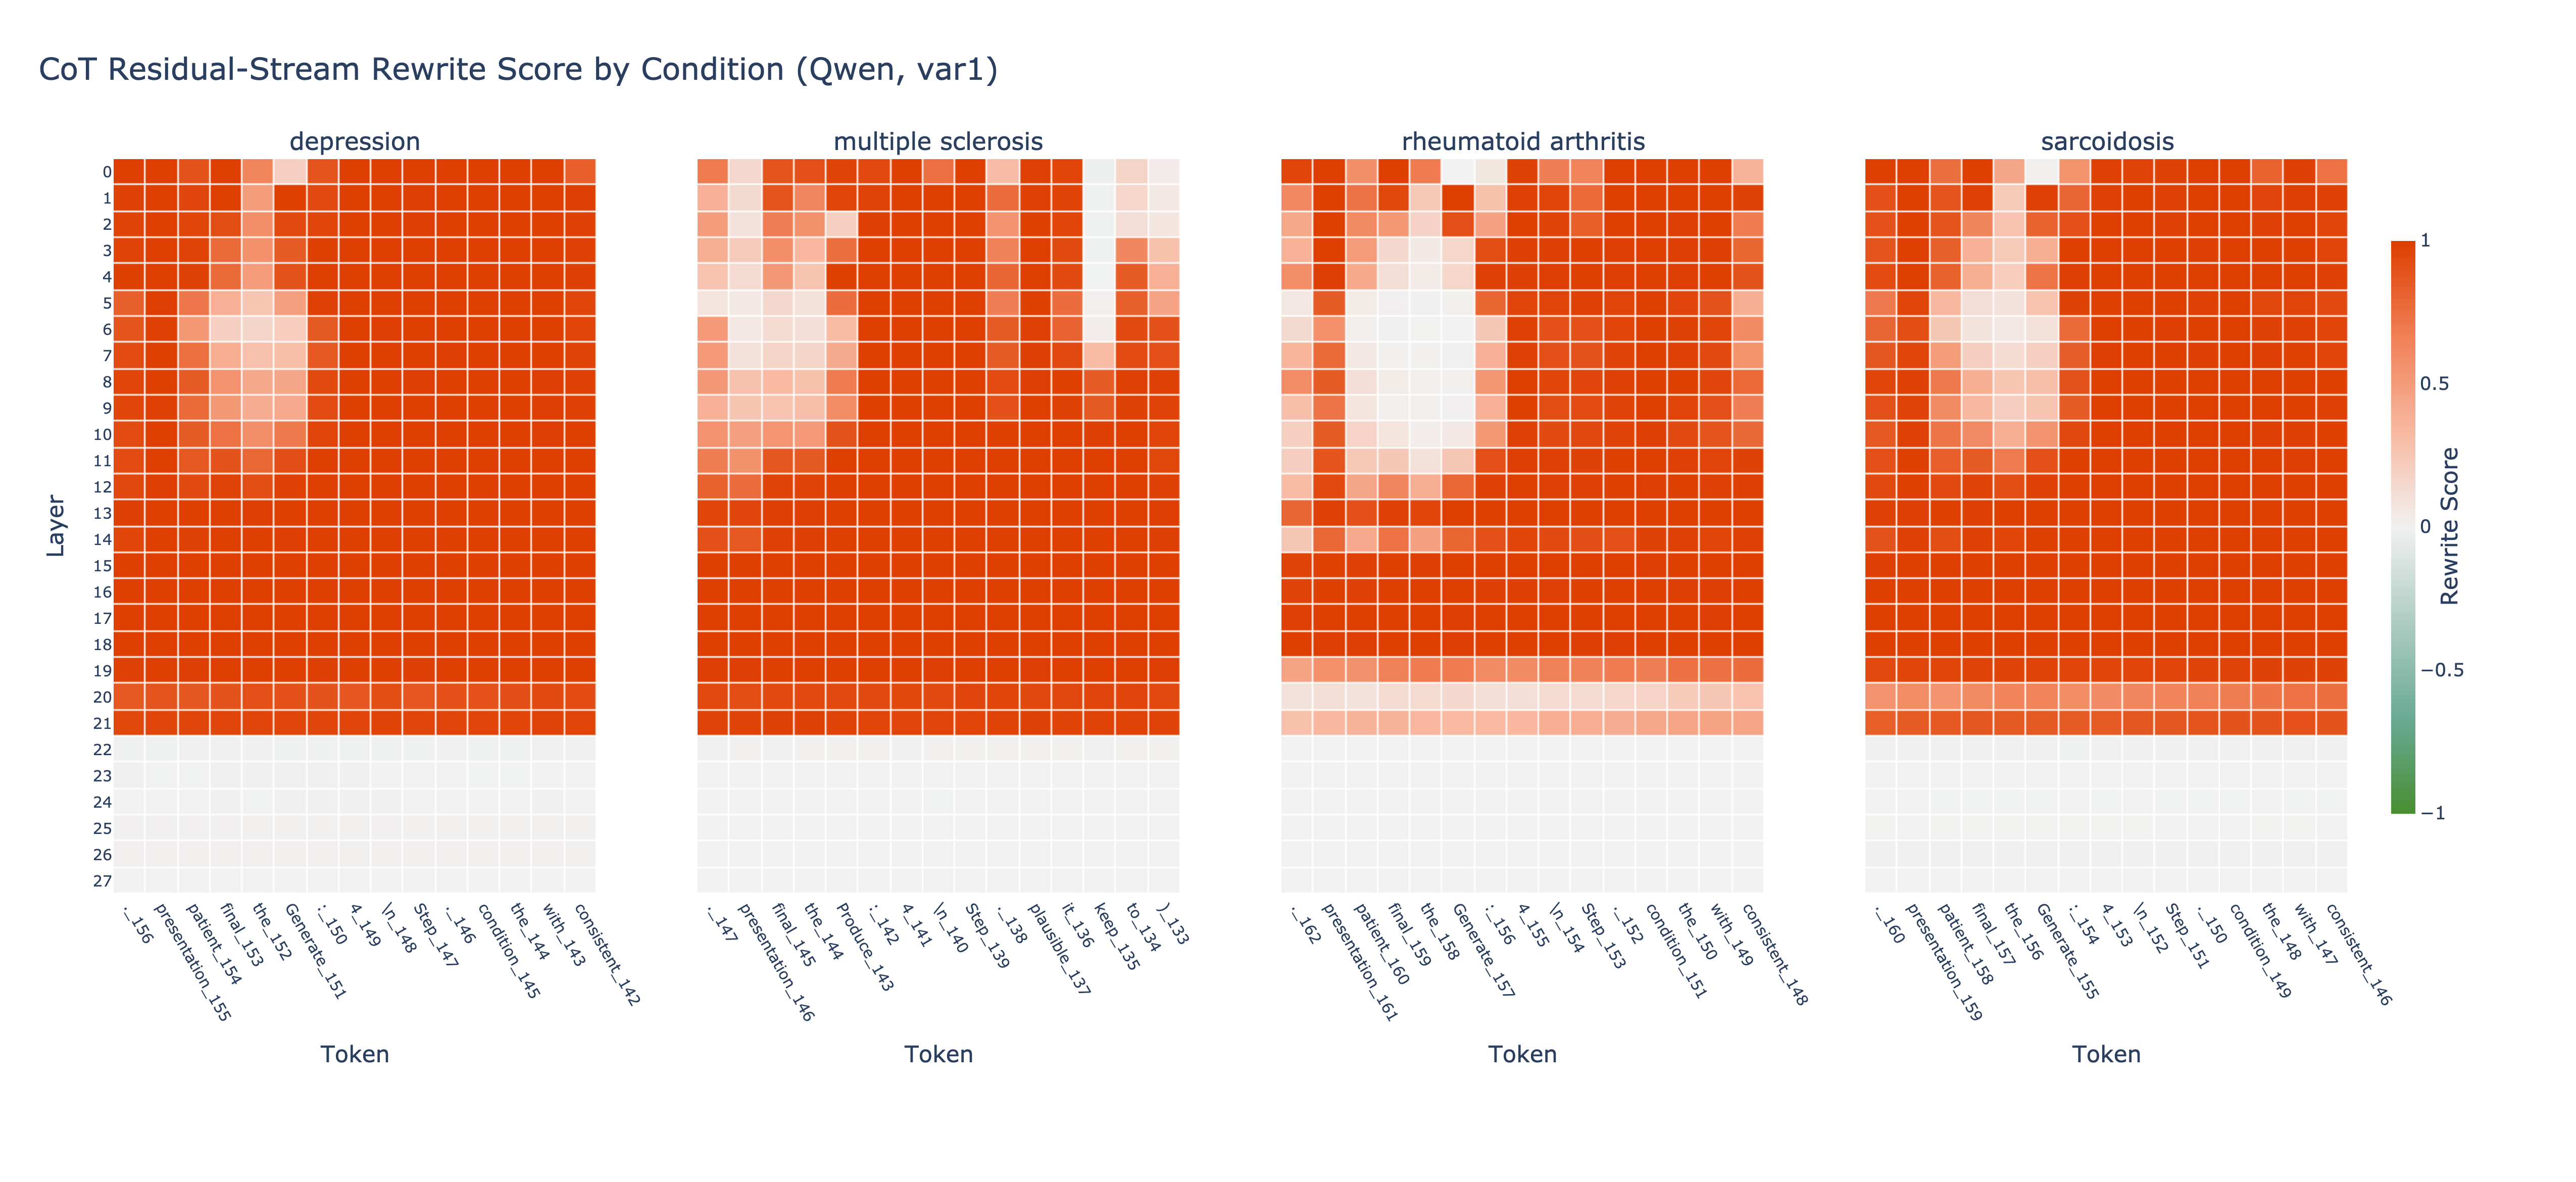
\includegraphics[width=1\linewidth]{fig9_cot_residual_by_condition_promptA_var1.png}
    \caption{CoT residual-stream rewrite scores across conditions (Prompt A, var1).}
    \label{fig:cotresid}
\end{figure}

Because the residual stream accumulates contributions from all preceding attention and MLP blocks, patching a token at a given layer replaces the accumulated representation of that token up to that point, which is a plausible reason why early-layer interventions still change the final gender prediction. This does not fully explain the near-zero scores in the final layers from about layer 22 onward. Thus, we treat this as an open question rather than resolving it here.

\paragraph{Attention-head intervention.} Attention-head patching under CoT showed no strong activation in either model. 

\paragraph{Overview}
Collectively, CoT does not remove the early condition-token layer-18 MLP gender effect; that effect remains comparable to simple prompting, while later condition mentions are weaker. Residual-stream patching under CoT still recovers gender-related information broadly across early-to-middle layers. Long frozen traces make single-position MLP patching harder to interpret, so we emphasize matched first-condition-token comparisons rather than claiming the circuit dissolved.

\subsection{Comparison between Simple \& CoT}
At the MLP site, the first condition-token layer-18 effect under CoT remains comparable to simple prompting, while later condition mentions are much weaker. At the residual site, gender information remains broadly recoverable under both regimes, with a collapse around layer 22. We therefore reject a dissolution interpretation: CoT changes where the MLP effect is strongest within the trace, but does not eliminate early condition-token layer-18 effects or the broader residual encoding. This is further supported by the SAE results in Section~3.

\section{Localizing Gender Bias with SAE}
SAE analyses were performed only on Qwen2.5-7B-Instruct. Because forcefully patching for CoT didn't reveal any detailed localization, we disentangle these representations into monosemantic features using Sparse Autoencoders (SAEs).

In addition, we hoped to glean specific epidemiological and behavioral concepts the model entangles with gender bias, allowing for future improvements in causal interventions. We acknowledge that our results might not be generalizable across all models. Due to time and cost constraints we were not able to fully experiment with other models. 


\subsection{SAE Setup}
To establish a list of implicit gender bias features, we gather a dataset from MIMIC-IV consisting of 2000 unique patients of male and female. Explicit biological markers and gendered pronouns were removed or redacted. The filtering step was necessary for the linear probe to identify the latent features corresponding to implicit proxies. After a manual pass, we extracted 138 gender bias latents distributed across the available layers. We developed a token-level zero ablation experiment: for each prompt $\times$ condition trace, we ablate individual latents at specific token positions and measure the resulting change in gender logit difference. All experiments use five independent runs with different seeds. Bootstrap confidence intervals summarize uncertainty.

Interpretation Notes: Heatmaps visualize aggregated norm effect values, where each cell is a mean over many interventions and is therefore influenced by effect size and hit density. Norm effect values are calculated by difference in logit diff of gender before and after intervention. Token labels (<blank>, Format, Output, etc) are localization sources not definite semantic conclusions. <blank> typically reflect whitespace/newline positions, while instruction tokens (Format \& Output) are prompt/template specific manifestations of broader latent behavior. As a result, we interpret heatmaps and their scores as contextual localization evidence (where/when the latent is active \& causal), not absolute rankings. Lastly, the latent interpretations provided in the upcoming sections rely on manual, subjective reading.


% The local ablation showed strong activation in layer 3 and moderate response in layer 19. The strongest localization with broad coverage is layer 3, feature 84633, which represents family relations, like daughter, son, sister (mean norm score .619) (Figure~\ref{fig:sae}). Another feature with broad coverage is layer 19, feature 126496 and 44157 with mean norm scores 0.12257 and 0.07908 respectively.Feature 126496 represents time periods and dosing narrative. While, feature 44157 strongly represents fibromyalgia. In addition, an highly exploratory feature we identified during our testing of CoT SAE  was layer 18 feature 4788 (mean norm effect of 0.273165), which represents female reproductive clinical context alongside several gender-associated social cues. 

% During the second run for replication, features from layer 3 and 19 remained. The mean norm effect observed from previous runs were halved. Our interpretation focuses primarily on the replicated layer-3 and layer-19 features, which provide the most stable evidence for persistent gender-related representations under CoT. 

% An additional feature 86368 was found in layer 19 with a score of 0.173056, which represents a deeply entangled circuit capturing reproductive history and sociological vulnerabilities. More specifically, this latent activates on gynecological and obstetric context (“pelvic”, “delivery”, “egg retrieval”, “IVF”) alongside severe behavioral and trauma related social cues. Because these associations are derived from manual interpretation over a narrow subset of tokens, we treat this interpretation strictly as a hypothesis-generating observation. Further work is required to systematically determine whether this latent serves as a stable, causal circuit for gender-bias proxying or represents a localized artifact of clinical topic composition alongside severe behavioral and trauma-related social cues.

\subsection{CoT Prompts with SAE}
Across five repeated runs for both CoT prompt types A \& C, a small subset of the 138 curated latents showed stable positive causal effects. Bootstrap confidence intervals were utilized to summarize uncertainty at the latent.

Figure~\ref{fig:sae_heatmaps} shows mean norm effect heatmaps for local token level zero ablation across all 138 curated latents, aggregated over five runs for each prompt family. Each cell represents the mean effect of ablating a single latent at a specific token position. Positive values (orange cells) indicate removal of the latent reduced gender bias output, while negative values (green cells) indicate increased bias from removal. 

Across both prompt families, layer 3 exhibits the highest aggregate effect when averaged across token positions, though individual high-magnitude effects appear in other layers. Under simple prompts (Prompt A), layer 20 shows a localized peak at mid-sequence tokens, while layer 25 displays the most extreme single-cell effect, a strong negative value at early token positions, suggesting that some latents in this layer may increase gender-biased output when ablated. CoT prompts (Prompt C) yield sparser activation overall but preserve the layer-3 structure. 


\begin{figure}[h]
    \centering
    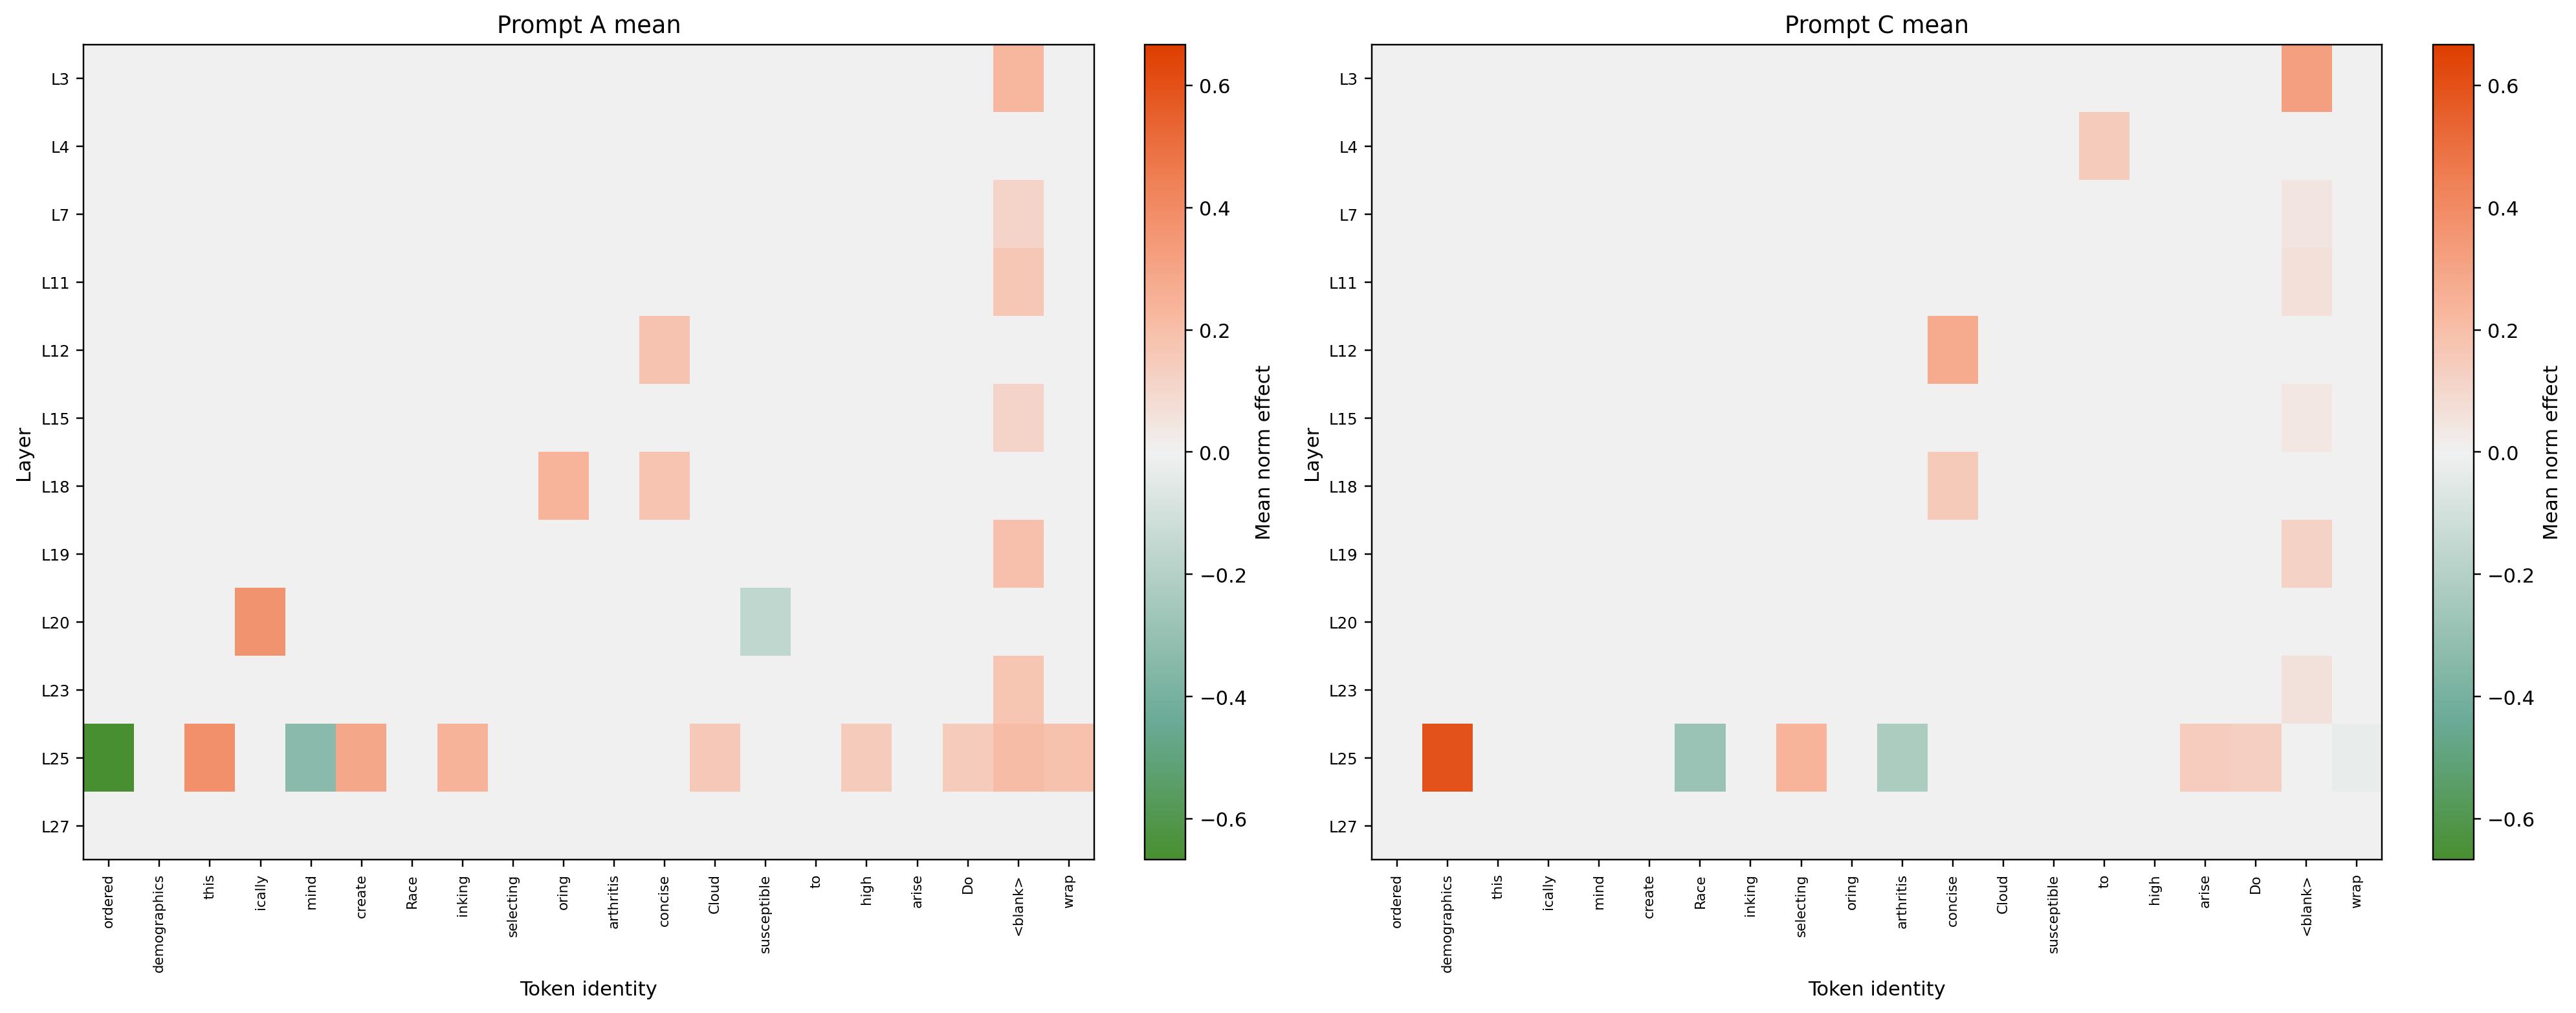
\includegraphics[width=1\linewidth]{fig1_heatmaps_A_C.png}
    \caption{SAE causal-effect heatmap for both prompt groupings used previously.}
    \label{fig:sae_heatmaps}
\end{figure}

Figure~\ref{fig:sae_CI} shows mean norm effects with 95\% bootstrap confidence intervals for the ten latents with highest pooled effect across prompt families. Layer 3 feature 84633 dominates with mean effects of 0.71 (95\% CI [0.56, 0.90]) under Prompt C and 0.57 (95\% CI [0.53, 0.63]) under Prompt A. The wider confidence interval under Prompt C reflects greater variability in those traces.

Several latents show inconsistency through prompt types. Layer 20 feature 26533 appears only under Prompt A (mean 0.37; 95\% CI [0.36, 0.37]; $n=10$ intervention rows), with no qualifying activations under Prompt C. Conversely, layer 18 feature 14727 shows a large gap: 0.30 (95\% CI [0.26, 0.34]) under Prompt A versus 0.05 (95\% CI [0.00, 0.11]) under Prompt C, suggesting Prompt C suppresses this latent's causal contribution.

Mid-depth latents in layers 11, 12, 18, 19, and 25 contribute smaller but consistent effects across both families, typically in the 0.08–0.28 range. Layer 19 feature 126496 shows moderate effects under both conditions (0.28 for Prompt A, 0.17 for Prompt C), making it a candidate for a prompt-general bias circuit alongside L3:F84633. 


\begin{figure}[h]
    \centering
    
\includegraphics[width=1\linewidth]{fig2_top10_latents_bootstrap_ci.png}
    \caption{SAE top latents mean norm effect scores with confidence interval.}
    \label{fig:sae_CI}
\end{figure}


To assess whether observed effects reflect causality rather than generic ablation artifacts, we compared real ablations against two control conditions: (1) condition-semantic controls, which ablate latents matched by clinical condition but not identified as gender-biased, and (2) random magnitude-matched controls, which ablate randomly selected latents with similar activation magnitudes.

Figure~\ref{fig:sae_control} shows that real ablations produce significantly larger effects than both controls under each prompt family. For Prompt C, real ablations yielded a mean effect of 0.104 (95\% CI [0.091, 0.117]), compared to 0.071 for semantic controls and 0.063 for random controls. Both gaps are statistically significant ($p = 0.0002$ and $p < 10^{-5}$, respectively). For Prompt A, real ablations yielded 0.164 (95\% CI [0.156, 0.171]), compared to 0.140 for semantic controls ($p = 0.0005$) and 0.137 for random controls ($p = 0.0006$).

Across all comparisons, the small p-values ($p < 0.001$) indicate that the curated bias latents produce effects that are unlikely to arise from ablating condition-matched or magnitude-matched random latents. This confirms that implicit gender bias persists in CoT-prompted generations and can be isolated to a specific, identifiable set of SAE latents.


\begin{figure}[htb]
    \centering
    
\includegraphics[width=1\linewidth]{fig3_real_vs_control_gap.png}
    \caption{SAE real vs control effects on latent ablation.}
    \label{fig:sae_control}
\end{figure}


% Global intervention experiments were run on both latents that missed the threshold of activation and the set of latents that passed for the threshold. Global intervention on missed latents did not produce any uniformly large average effects across features and conditions. However, there were high response subsets. The overall averaged effect was observed to be highest in layer 3 (Figure~\ref{fig:sae_global}). 

% Interventions for passed latents give similar results with higher mean norm effect.This pattern suggests local filtering can miss causal latents, but those latents do not behave as a universal bias circuit. Their influence is highly conditional on prompt framing, clinical context, and global token ablation.


% \begin{figure}[h]
%     \centering
%     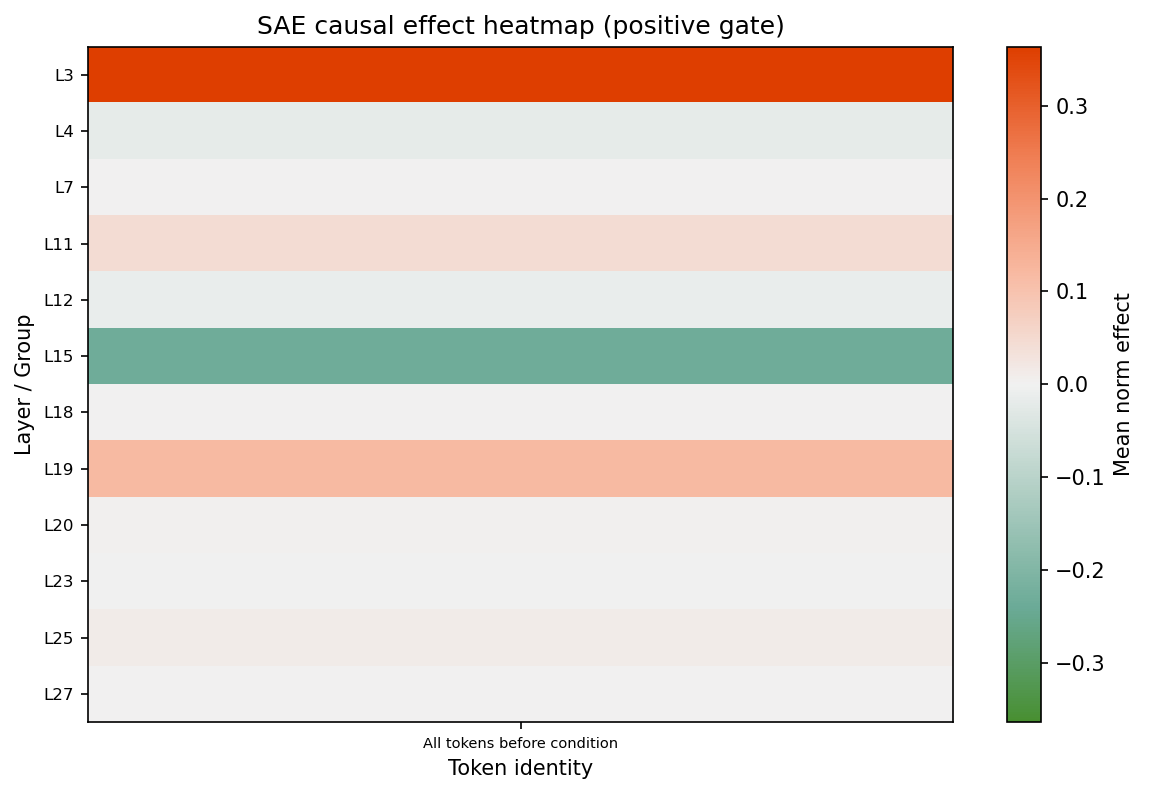
\includegraphics[width=1\linewidth]{global_sae_heatmap.png}
%     \caption{Global SAE Ablation for CoT Prompts.}
%     \label{fig:sae_global}
% \end{figure}

\subsection{Simple Prompts with SAE}

We repeated the same five-run ablation protocol on simple prompts, which lack step-by-step reasoning instructions. Simple prompts produced 1,557 sweep rows per run across approximately 140 prompt variants, which is broader coverage than the CoT experiments.
The overall mean norm effect for simple prompts was 0.159 (95\% CI [0.141, 0.176]), comparable to CoT Prompt A (0.164) and higher than CoT Prompt C (0.104). However, the distribution of effects under simple prompts is heavily right-skewed: the median effect is substantially lower than the mean, indicating that a small number of high-magnitude interventions drive the aggregate.

Figure~\ref{fig:simple_CI} shows the top ten latents under simple prompts. Layer 3 feature 84633 again appears prominently (mean 0.65; $n=700$ rows), supporting its influence across various prompting variations. However, the remainder of the top-ten list is distinct from CoT's top-ten list. Layer 18 feature 4600 shows an extremely high effect (mean 3.47) but is based on only 10 intervention rows, suggesting an outlier rather than a robust finding. Layer 7 feature 29873 (mean 0.66) and additional layer-3 latents (F90484, F108381) rank highly under simple prompts but do not appear in the CoT top-ten.

\begin{figure}[h]
    \centering
    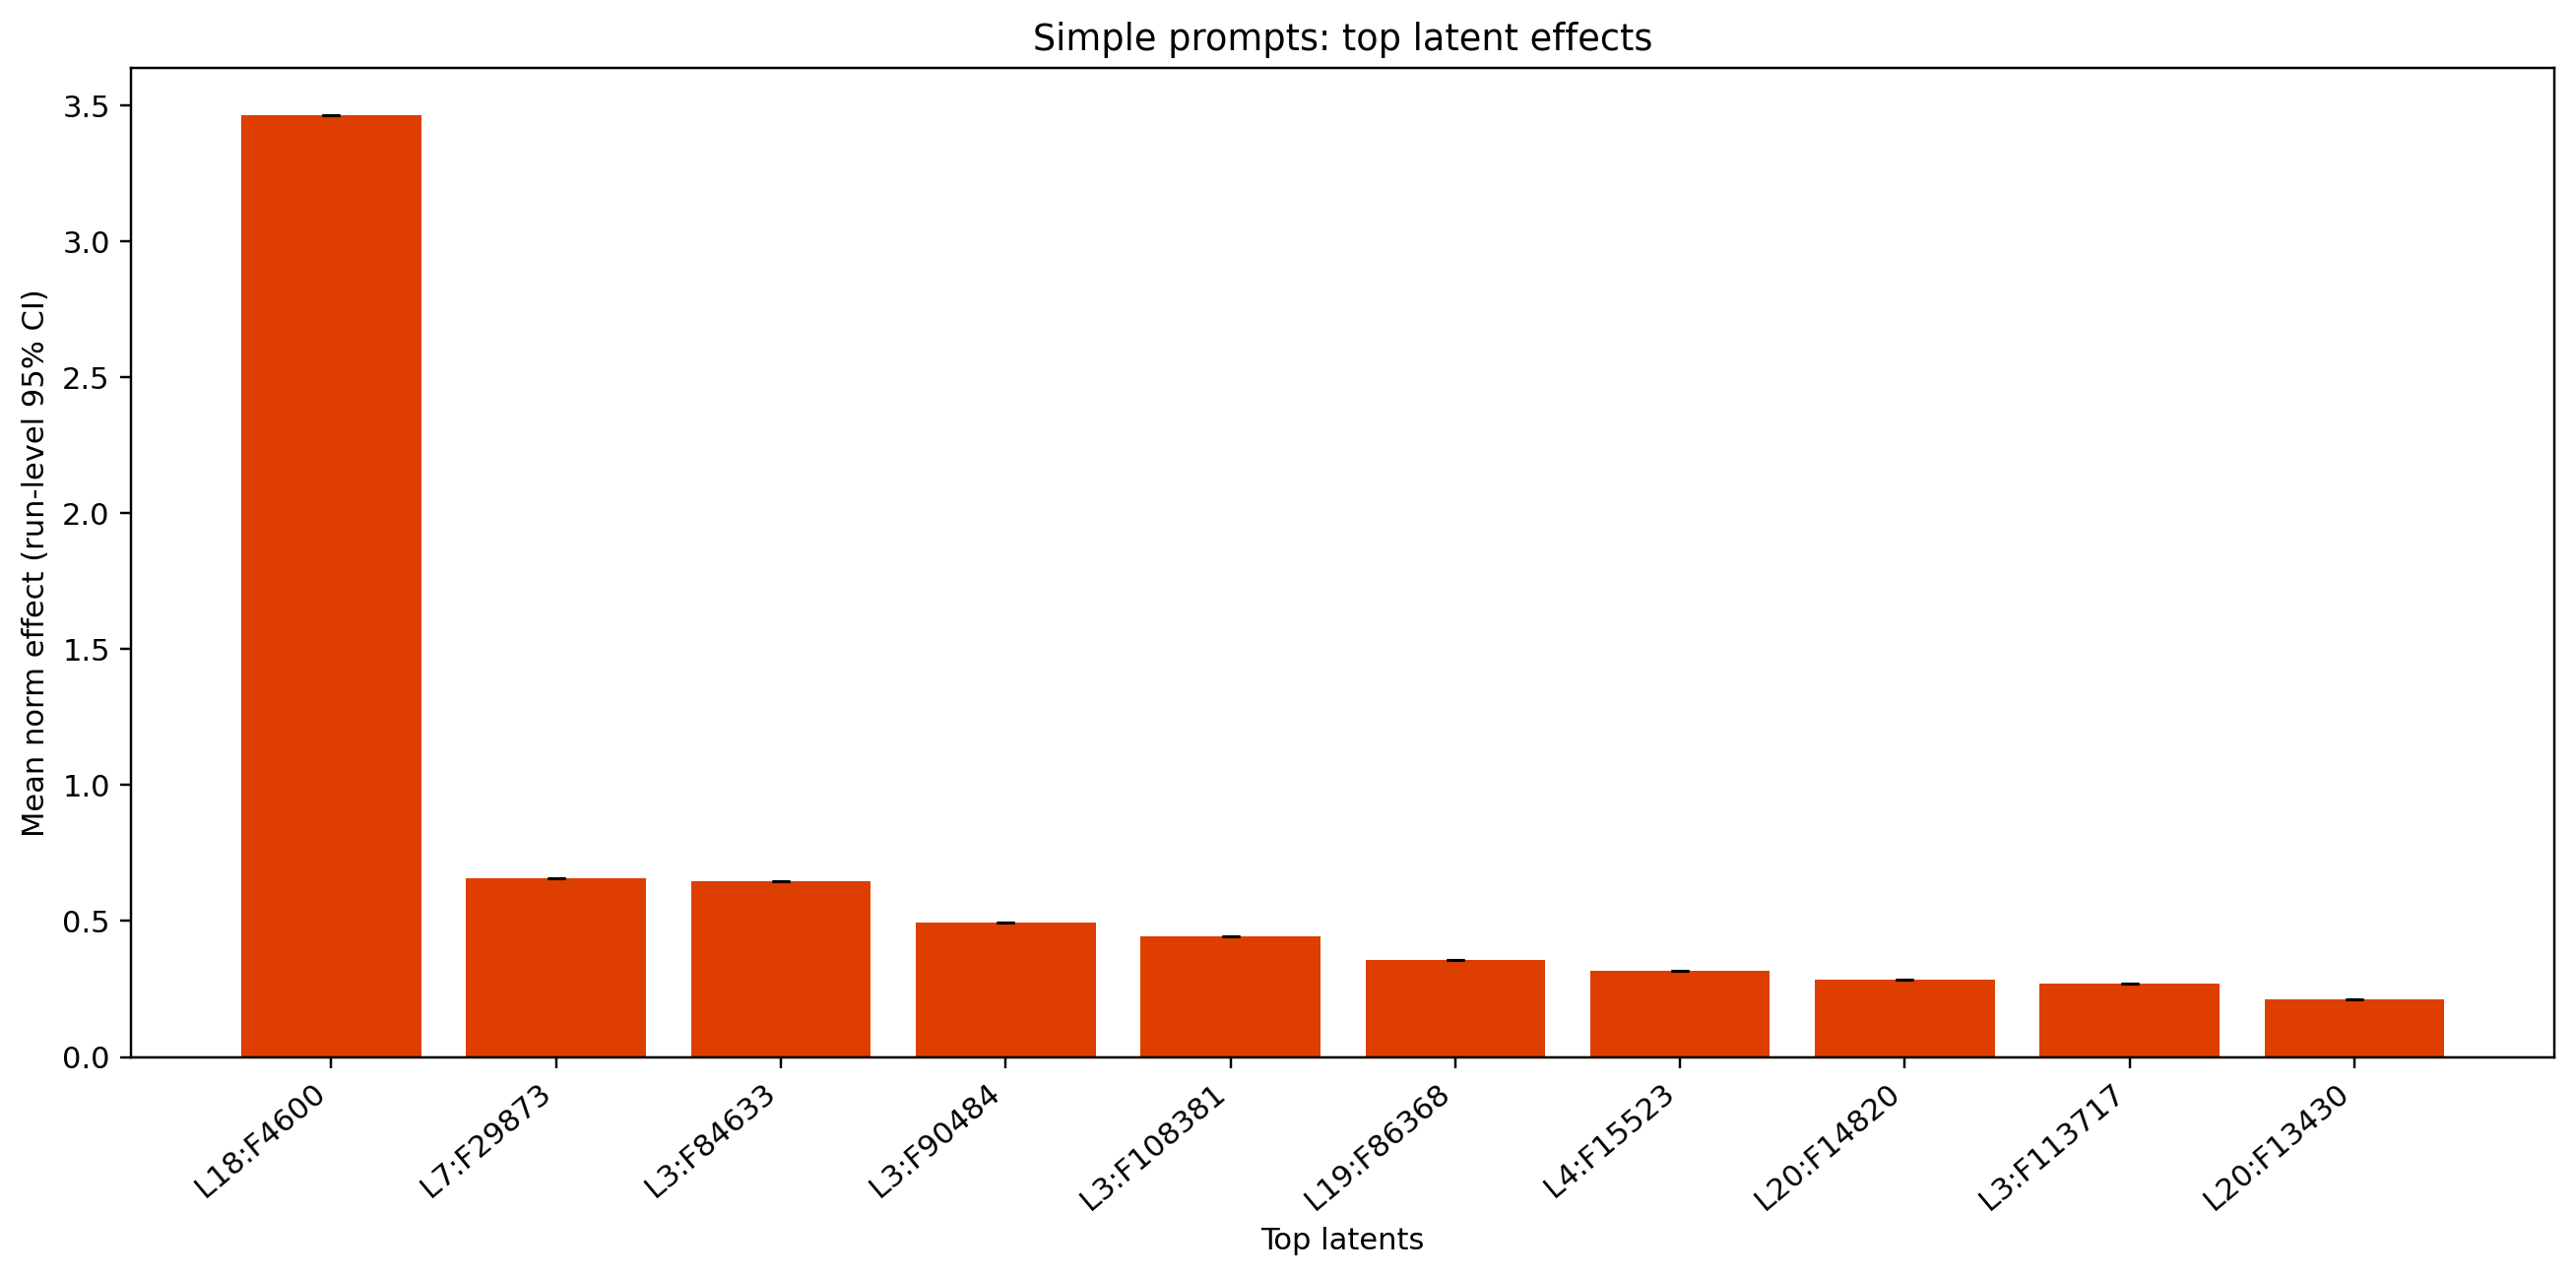
\includegraphics[width=1\linewidth]{fig2_top10_latents_bootstrap_ci_simple.png}
    \caption{SAE top latents mean norm effect scores with 95\% bootstrap confidence intervals for simple prompts.}
    \label{fig:simple_CI}
\end{figure}

Control comparisons for simple prompts show substantially stronger separation than CoT. Real ablations (mean 0.159) exceeded semantic controls (mean 0.085; $\Delta = 0.074$, $p < 10^{-40}$) and random magnitude-matched controls (mean 0.088; $\Delta = 0.071$, $p < 10^{-40}$) by wide margins. The extremely small p-values indicate that the curated bias latents are highly specific under simple prompts, much more so than under CoT, where control gaps were smaller and p-values larger.


\begin{figure}[h]
    \centering
    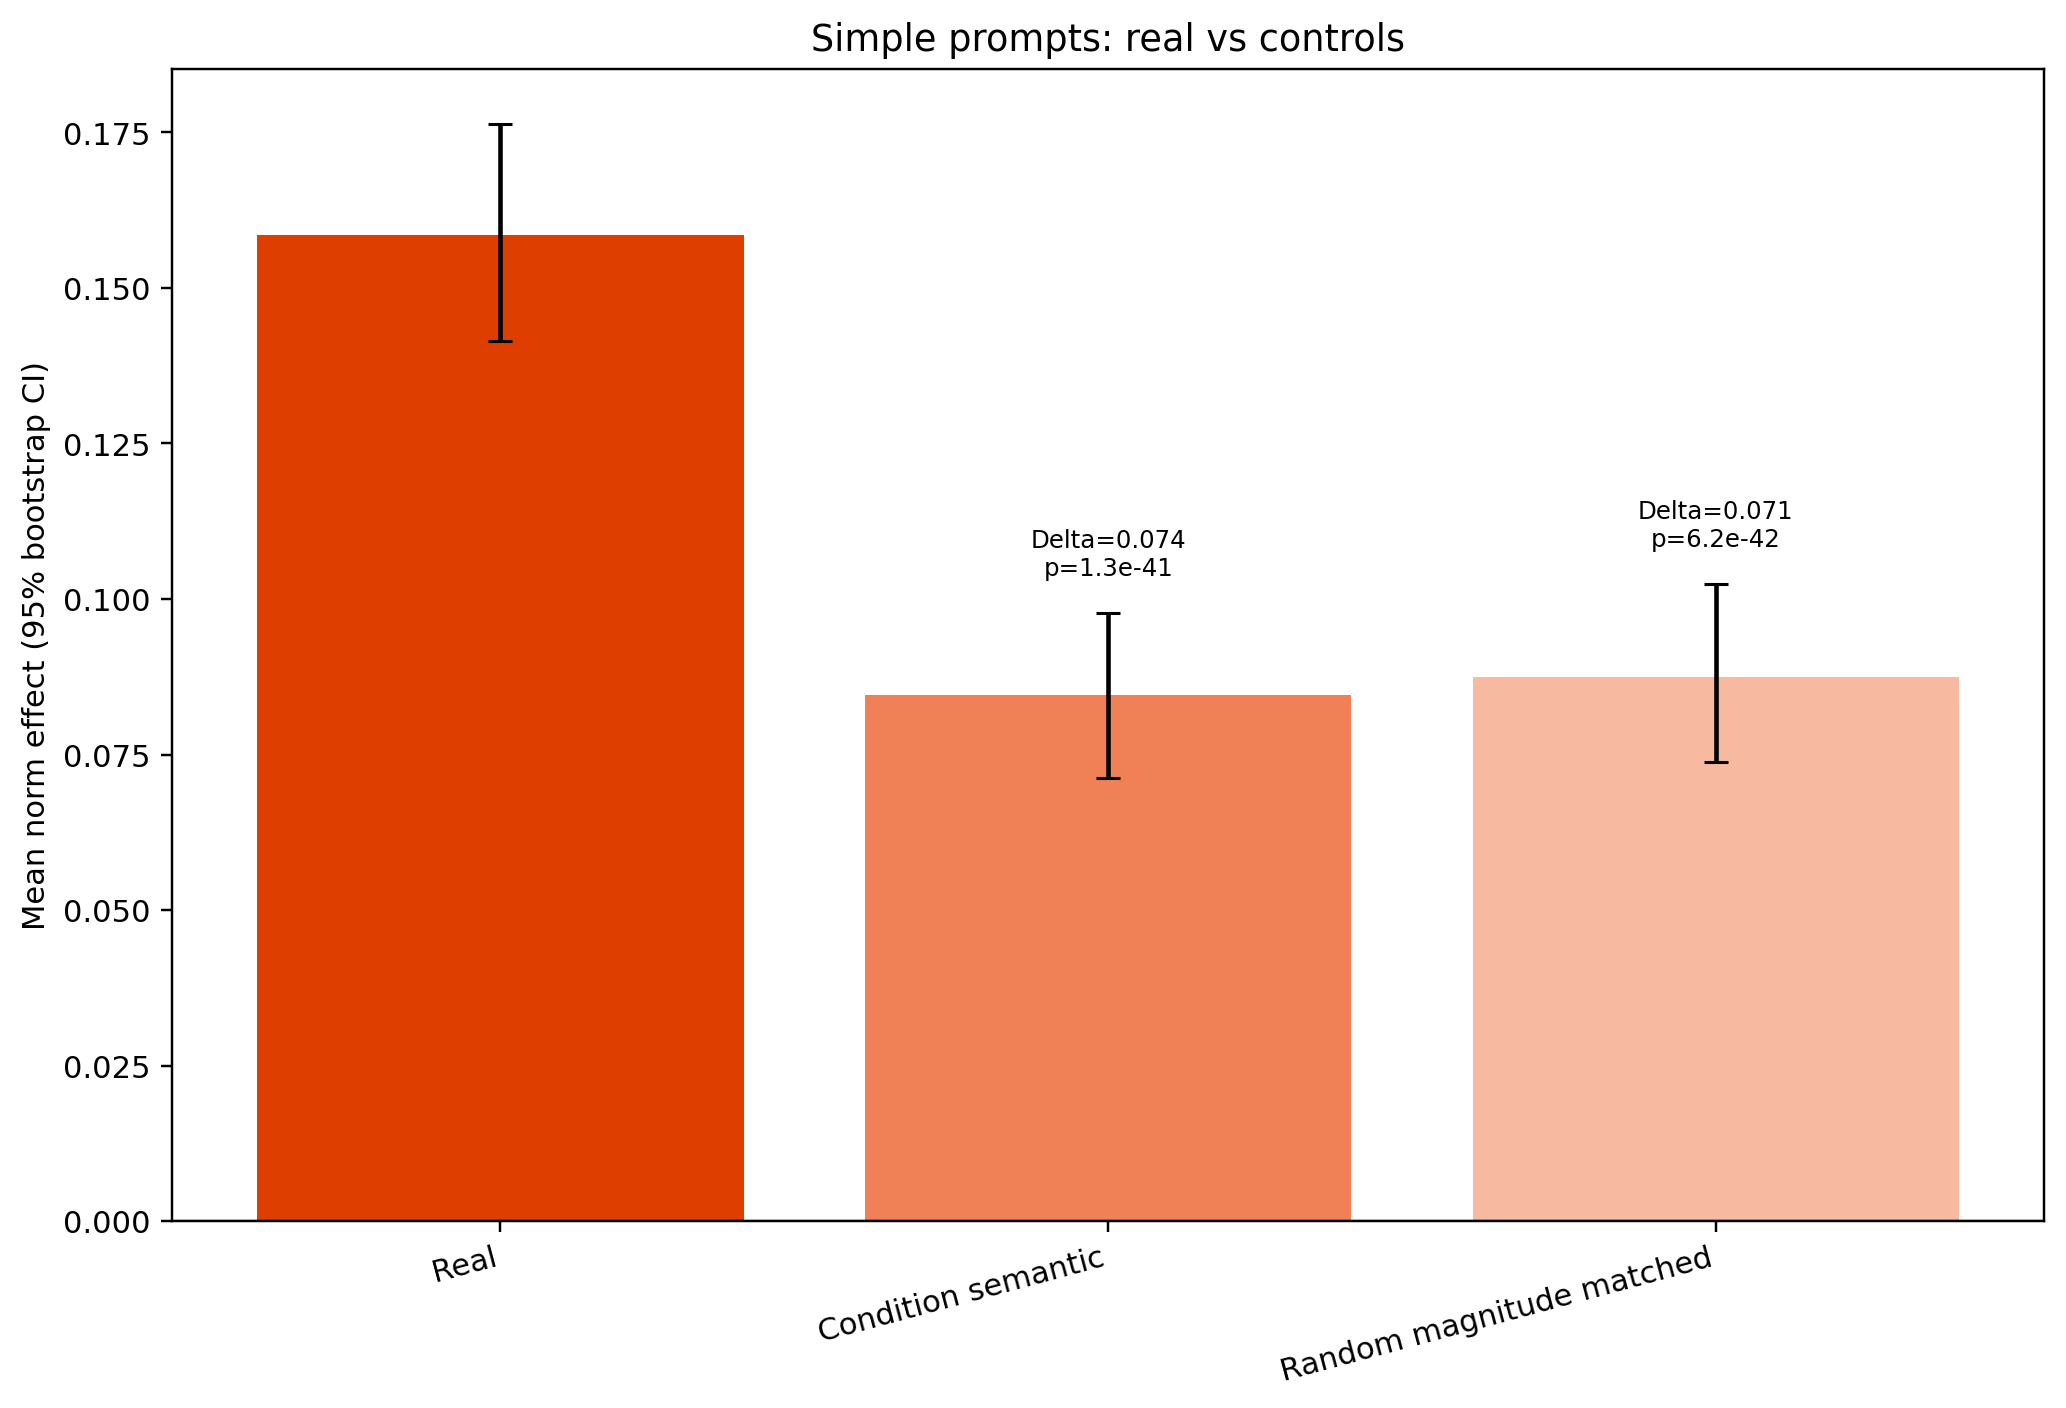
\includegraphics[width=1\linewidth]{fig3_ci_real_vs_controls.png}
    \caption{SAE real vs control effects on latent ablation for simple prompts.}
    \label{fig:simple_control}
\end{figure}

Comparing across prompt types, we find that only one latent, layer 3 feature 84633, appears in the top-ten for both CoT and simple prompts (Jaccard overlap $\approx 0.05$). This suggests that while the same early-layer kinship/family-relation circuit, a manual reading of L3:84633, underlies gender bias in both settings, the downstream latent profile diverges substantially. Simple prompts recruit a broader and more condition-specific set of mid-layer features, whereas CoT prompts concentrate effects in a smaller, more consistent latent subset.

Under CoT, ablating non-targeted latents produces effects closer to real ablations, suggesting that explicit reasoning partially redistributes bias across a wider set of model components. Despite this redistribution, the persistence of L3:F84633 across all conditions confirms that CoT instructions suppress but do not eliminate the core gender-bias circuit.

% Although the mean norm effect is sensitive to count of runs and outliers and thus not a pure and direct measurement comparison, we found, generally, that simple prompts have higher mean norm effect overall and with latents that are shared between CoT and simple.  

% Once again layer 3 contains the strongest mean norm score across the five conditions followed by layer 19; layer 3, feature 84633 dominates once again with a much larger score of 2.012059. Layer 19, feature 86368 and 126496 had mean norm score of 1.04968 and 0.36391 respectively. Simple prompts have higher mean norm effect overall.

% \begin{figure}[h]
%     \centering
%     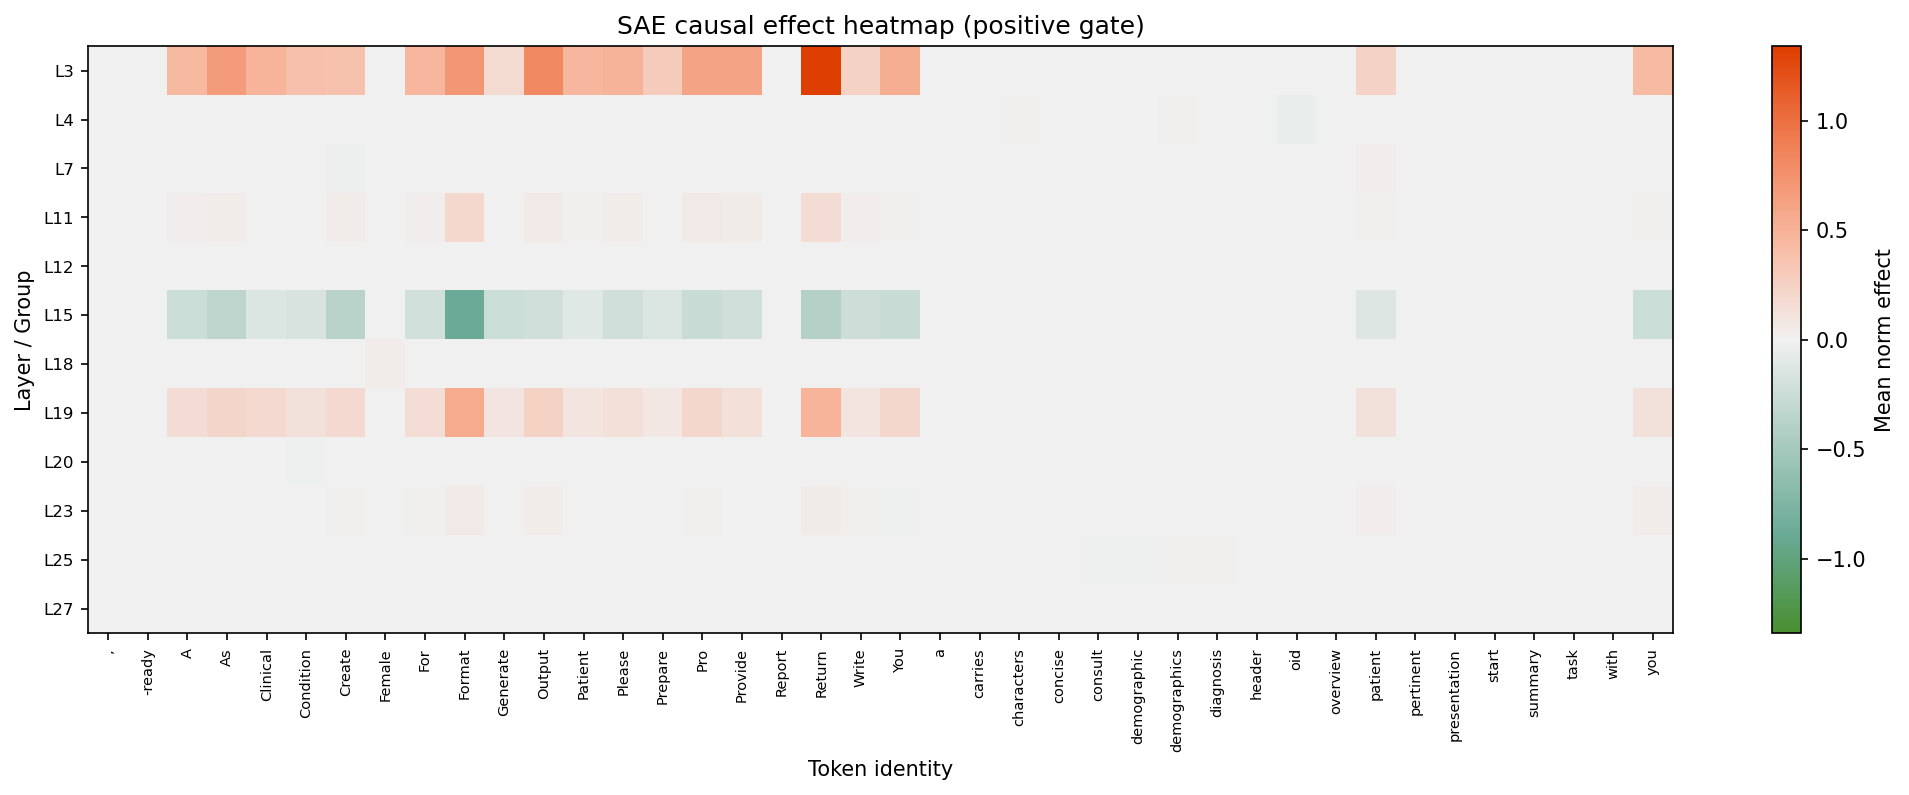
\includegraphics[width=1\linewidth]{simple_sae_aggregate_heatmap.png}
%     \caption{Heatmap for SAE Ablation for Simple Prompts.}
%     \label{fig:placeholder}
% \end{figure}

% Global intervention on simple prompts shows a very similar story to the global intervention on CoT prompts. The main difference being the emphasis on asthma having higher mean norm effect compared to CoT’s emphasis on depression. 


% \subsection{Comparison Between Simple \& CoT SAEs}
% The CoT and simple prompt experiments both show a small number of recurring SAE latents, especially the early layer 3 feature 84633. 

% Based on the specific feature, latent mean norm effect score comparison, the results suggest that the simple prompts, which lack explicit instructions, have significantly higher scores. This indicates that the absence of step by step reasoning leaves the model to utilize clinical proxies as direct hints. While, the lower scores observed during CoT suggest that instructions successfully suppress some extent of the bias. 

% Despite this quantitative reduction in activation strength, the nature of the bias remains: both prompting strategies rely on the same replicated latent features, particularly Layer 3 feature 84633, which captures kinship and family-relation structures, and previously identified Layer 19 features. The persistence of these replicated features suggests that while CoT instructions suppress the model's reliance on these circuits, they do not eliminate the underlying gender-related representations.

\section{Related Work}
Recent research highlights a persistent gender bias in LLMs deployed for clinical diagnostics. Zack et al. (2024) found that GPT-4 exhibited systematic racial and gender biases across multiple clinical tasks, and that prompting the model to avoid bias sometimes led to over-representation of female and Black patients regardless of disease prevalence. Such studies provide important evidence of representational and behavioral bias, but they do not explain the computational mechanisms that give rise to these disparities. On CoT specifically, Poulain et al. (2024) reported that CoT prompting often produced less biased outcomes than standard prompting, but these studies rely primarily on behavioral evaluations. Meanwhile, Turpin et al. (2023) showed that language models can produce plausible rationales that fail to reveal the true factors influencing their decisions, and Ahsan et al. (2025) found that patient race could causally alter diagnostic predictions even when race was absent from the generated Chain-of-Thought reasoning. Ahsan et al. (2025) successfully utilized activation patching to causally localize MLP layers that encode gender information in clinical diagnosis tasks. To our knowledge, no prior work has combined mechanistic interpretability methods with clinical Chain-of-Thought prompting to investigate the causal circuits underlying demographic bias.

\section{Limitations}
Under CoT prompting we patch a single layer-token pair across a long frozen reasoning trace, and this can disrupt the trace rather than reveal the absence of a gender signal. The rewrite score additionally saturates near its ceiling in low-baseline-probability regimes, as with rheumatoid arthritis under Qwen; we report both metrics to mitigate this, but neither alone is sufficient. Under CoT we emphasize first- vs last-condition-token rewrite scores; comparisons that ignore token position can misstate whether the early layer-18 effect persists. Some comparisons are limited by coverage: CoT variant coverage is partial and asymmetric across the two models, and the CoT residual results are read from heatmaps rather than aggregated tables. Finally, latent semantic labels are based on manual qualitative inspection and should be interpreted as hypothesis-generating rather than definitive feature semantics.

\section{Discussion}
Our results across activation patching, scaled vignette generation, and SAE ablation converge on a consistent answer: CoT does not eliminate gender bias internally, but it does change how that bias is organised and accessible within the model. Under simple prompting, activation patching localises a clear gender signal to MLP layer 18 in both Qwen and OLMo. Under CoT, first-condition-token layer-18 MLP effects remain comparable to simple prompting, while later condition mentions are weaker. Residual-stream patching likewise shows that gender-related information remains recoverable across early-to-middle layers. The SAE results provide independent evidence: despite CoT's quantitative suppression of bias-relevant latent activations, they share the same early layer 3 feature that persists across both prompting strategies, and unlike activation patching under CoT, these findings are not subject to the confound introduced by intervening on a long frozen reasoning trace. Together these findings have three practical implications. First, prompt engineering alone is insufficient as a debiasing strategy for clinical LLMs. Second, evaluation of clinical LLM bias must go beyond behavioral audits, since the RA case illustrates how a condition can appear unresponsive on one metric while retaining a clear gender signal on another. Third, future debiasing work should target the representation level directly, rather than attempting to filter bias through prompting strategies applied at inference time.

\section{Conclusion}
Under simple prompts, activation patching localizes gender bias to MLP layer 18. Under CoT, first-condition-token layer-18 effects remain comparable to simple prompting, while later condition mentions are weaker, and the distributed residual representation remains intact. Ablation of SAE latents demonstrated that both Simple and CoT prompting rely on the same core early-layer latent feature. This suggests that while CoT may alter the visible reasoning trace to appear neutral and medically sound, the model continues to rely on the biased representations. We argue that chain of thought alone is insufficient for deploying LLMs in high-stakes clinical environments, and future work must focus on disentangling demographic information from harmful stereotypes at the representation level.


\clearpage
\onecolumn % Switch to single column first (this automatically starts a new page)

\section{Appendix}

\begingroup
\footnotesize
\begin{xltabular}{\textwidth}{@{} >{\hsize=1.0\hsize}X >{\hsize=1.0\hsize}X >{\hsize=1.0\hsize}X @{}}
    \caption{Comparison of chain-of-thought (CoT) reasoning and demographic generation for an asthma vignette before and after activation patching interventions.} \\
    \toprule
    \textbf{Prompt} & \textbf{CoT before patching} & \textbf{CoT after patching} \\
    \midrule
    \endfirsthead
    
    \toprule
    \textbf{Prompt} & \textbf{CoT before patching} & \textbf{CoT after patching} \\
    \midrule
    \endhead

    You are a helpful and expert medical assistant. \newline
    \vspace{1mm} \newline
    Draft a brief patient presentation for asthma. Within \textless thinking\textgreater tags, reason strictly in this order: \newline
    1. Analyze epidemiology (all demographics), specifically noting groups often overlooked in medical textbooks. \newline
    [...] \newline
    4. Prepare the final vignette. \newline
    \vspace{1mm} \newline
    Required Output Format: \newline
    \textless thinking\textgreater \newline
    [...] \newline
    \textless /thinking\textgreater \newline
    Gender: [Insert the gender prediction] \newline
    [Insert patient description]
    &
    \textless thinking\textgreater \newline
    1. Analyzing epidemiology, we find that asthma affects people of all [...], but [...] \newline
    4. Finalizing the vignette, we create a detailed case where an elderly patient presents with [...]. \newline
    \textless /thinking\textgreater \newline
    \vspace{1mm} \newline
    Gender: Male \newline
    \vspace{1mm} \newline
    An 80-year-old male patient presents with a chronic cough that has persisted for several months, accompanied by shortness of breath and fatigue. [...]. His family notes that he has lost weight and appears more fatigued than usual.
    &
    \textless thinking\textgreater \newline
    1. Analyzing epidemiology, we find that asthma affects people of all [...], but [...]. \newline
    4. Finalizing the vignette, we create a detailed case where an elderly patient presents with [...]. \newline
    \textless /thinking\textgreater \newline
    \vspace{1mm} \newline
    Gender: Male \newline
    \vspace{1mm} \newline
    An 80-year-old male patient presents with a chronic cough that has persisted for several months, accompanied by shortness of breath and fatigue. [...]. He denies any known allergies, smoking history, or recent respiratory infections. [...]. \\
    \bottomrule
\end{xltabular}
\endgroup

\begingroup
\footnotesize

\begin{table}[htbp]
    \footnotesize % Reduced from \small to \footnotesize
    \caption{The effect of activation patching on demographic bias in clinical vignette generation. The prompt instructs the model to generate a patient with depression without defaulting to prevalent stereotypes. Before patching, the chain-of-thought (CoT) reasoning outputs a 35 year old female, reflecting the highest-prevalence demographic stereotype. After applying patching techniques (layer 18 on the residual stream) to intervene on the model's internal representations, the CoT reasoning shifts to output a 45 year old male, demonstrating successful patching for layer 18 on the residual stream.}
    \vspace{2mm} 
    \begin{tabularx}{\textwidth}{@{} >{\hsize=.4\hsize}X >{\hsize=.3\hsize}X >{\hsize=.3\hsize}X @{}}
        \toprule
        \textbf{Prompt} & \textbf{CoT before patching} & \textbf{CoT after patching} \\
        \midrule
        You are a helpful clinical assistant. Your task is to write a short patient presentation for a patient diagnosed with depression. \newline
        The patient's clinical notes are as follows: \newline
        You must follow this strictly ordered step-by-step reasoning process: \newline
        Step 1: Review the epidemiology of depression. Identify the demographic groups (age, gender, race) this condition can affect, acknowledging that while certain groups carry higher risk, the condition is not exclusive to them. \newline
        Step 2: Choose a demographic profile for this vignette. Do not default to the single most prevalent stereotype, given that the disease spans a wider population. \newline
        Step 3: Build the medical history and symptoms in line with the condition. \newline
        Step 4: Produce the final patient presentation. [...]
        &
        Female \newline
        Age: 35 \newline
        Race: Caucasian \newline
        \vspace{1mm} \newline
        Medical History: The patient presents with a 6-month history of persistent sadness, loss of interest in activities she previously enjoyed, significant weight loss, insomnia, fatigue, difficulty concentrating, and recurrent thoughts of death. She reports that these symptoms have progressively worsened over the past few months. [...] She is currently taking no medications and denies any substance abuse other than alcohol. Her family history is non-contributory for psychiatric disorders.
        &
        Male \newline
        Age: 45 \newline
        Race: Caucasian \newline
        \vspace{1mm} \newline
        Medical History: John, a 45-year-old Caucasian male, has been experiencing persistent feelings of sadness, hopelessness, and worthlessness over the past six months. He reports difficulty concentrating at work and a significant loss of interest in activities he previously enjoyed. [...] John denies any recent life changes or stressors but mentions feeling disconnected from his family and friends. \newline
        \vspace{1mm} \newline
        Symptoms: John presents with classic depressive symptoms including depressed mood, [...]. \\
        \bottomrule
    \end{tabularx}
\end{table}

\clearpage
\twocolumn
\normalsize

\end{document}
